\documentclass[12pt]{article}

\usepackage{sbc-template}
\usepackage[T1]{fontenc}
\usepackage[utf8]{inputenc}
\usepackage[brazil]{babel}
\usepackage{graphicx,url}
\usepackage{amsmath,amssymb}
\usepackage{booktabs,longtable,array}
\usepackage{tikz}
\usetikzlibrary{positioning,arrows.meta,calc,babel}

\sloppy
\graphicspath{{figuras/}}

% Tabelas mantêm a fonte definida; reduzem somente quando excedem a largura do texto.
\newsavebox{\SBCtablebox}
\newenvironment{sbcfitwidth}{\begin{lrbox}{\SBCtablebox}}{%
  \end{lrbox}%
  \ifdim\wd\SBCtablebox>\linewidth
    \resizebox{\linewidth}{!}{\usebox{\SBCtablebox}}%
  \else
    \usebox{\SBCtablebox}%
  \fi}
\newcommand{\ind}{\mathbf{1}}

\title{Segmentação temporal de estruturas no sistema de reação--difusão de Gray--Scott: pré-processamento, arquiteturas e pós-processamento}

\author{Andre Luis Aguiar do Nascimento\inst{1}, Joao Guilherme Miranda Lago\inst{1},\\ Wesley dos Santos Gatinho\inst{1}}

\address{Universidade Federal do Maranhão (UFMA)\\
  Av. dos Portugueses, 1966 -- Bacanga, São Luís -- MA, 65080-805, Brasil
  \email{andre.aguiar@discente.ufma.br, jglago10@gmail.com, wesley.gatinho@discente.ufma.br}
}

\begin{document}

\maketitle

\begin{abstract}
This work evaluates how pre-processing, segmentation architecture and post-processing affect the segmentation of active-reaction regions in the Gray--Scott system of The Well. Ten pre-processing methods, three architectures (U-Net, SegFormer and Mask2Former) and five post-processing methods were applied to all 1,200 trajectories, segmenting from the substrate $A$ a ground truth obtained by Otsu thresholding of species $B$. On 120 test trajectories, U-Net reached a Dice of 0.953, against 0.892 for SegFormer, 0.768 for Mask2Former and 0.888 for Otsu thresholding of $A$. Pre-processing changed Dice by at most 1.37 percentage points, temporal filtering lowered it by 8.6 to 11.3 points, and the largest gains came from the random initial frame: excluding it, threshold optimization lowered the Dice of U-Net.
\end{abstract}

\begin{resumo}
Este trabalho avalia como o pré-processamento, a arquitetura de segmentação e o pós-processamento afetam a segmentação das regiões de reação ativa no sistema de Gray--Scott do The Well. Dez pré-processamentos, três arquiteturas (U-Net, SegFormer e Mask2Former) e cinco pós-processamentos foram aplicados às 1.200 trajetórias, que segmentam, a partir do substrato $A$, uma referência obtida pela limiarização de Otsu da espécie $B$. Em 120 trajetórias de teste, a U-Net obteve Dice de 0,953, contra 0,892 da SegFormer, 0,768 do Mask2Former e 0,888 da limiarização de Otsu em $A$. O pré-processamento alterou o Dice em no máximo 1,37 ponto percentual, o filtro temporal o reduziu em 8,6 a 11,3 pontos, e os maiores ganhos vieram do instante inicial aleatório: excluído esse instante, a otimização do limiar reduziu o Dice da U-Net.
\end{resumo}

%% =====================================================================
\section{Introdução}
\label{sec:introducao}

Sistemas de reação--difusão descrevem substâncias que se espalham no espaço enquanto reagem entre si. Quando as espécies difundem com velocidades diferentes, a difusão, que isoladamente suaviza qualquer perturbação, pode desestabilizar um meio homogêneo e dar origem a manchas, labirintos e ondas que surgem sem comando externo. Turing (1952) propôs esse mecanismo para explicar a morfogênese, e o mesmo arcabouço foi usado para descrever padrões biológicos \cite{kondo2010,murray2003} e foi observado experimentalmente em reatores químicos \cite{lee1993}. O modelo de Gray--Scott é a forma mínima desse fenômeno: duas espécies, uma reação autocatalítica cúbica e dois parâmetros de controle bastam para gerar padrões estacionários e dinâmicos qualitativamente distintos \cite{gray1983,pearson1993}. Para analisar um padrão desse tipo, não basta observar o campo de concentrações. É preciso responder onde estão as estruturas de interesse e como elas evoluem ao longo do tempo, o que exige transformar o campo contínuo em regiões, isto é, segmentá-lo.

A coleção The Well disponibiliza simulações do sistema de Gray--Scott, entre outros sistemas físicos, para o desenvolvimento de métodos de aprendizado de máquina \cite{ohana2024well}. Nesse conjunto, os modelos de referência são substitutos neurais, como o Fourier Neural Operator, que preveem os próximos estados do campo \cite{li2021fno}. A previsão, porém, não localiza as estruturas nem mede sua formação, migração ou extinção. A segmentação semântica por redes profundas, consolidada em imagens naturais e médicas \cite{long2015fcn,ronneberger2015unet,xie2021segformer,cheng2022mask2former}, oferece essa representação, mas seu comportamento em campos físicos simulados é menos documentado. Esses campos não têm textura nem cor, o domínio é periódico, e as estruturas aparecem, se dividem e desaparecem entre os instantes. Além disso, etapas clássicas de processamento de imagens que antecedem a rede, como normalizações e filtros de suavização, ou que a sucedem, como a escolha do limiar e a morfologia matemática, costumam ser aplicadas sem que se meça se e por que alteram a segmentação.

Nesse contexto, este trabalho avalia o efeito do pré-processamento, da arquitetura de segmentação e do pós-processamento sobre a segmentação temporal das regiões de reação ativa no sistema de Gray--Scott do The Well. O estudo segue um protocolo comum a uma turma de Processamento Digital de Imagens, no qual cada participante aplica o mesmo experimento a um sistema físico bidimensional diferente: dez pré-processamentos, três arquiteturas e cinco pós-processamentos, com entrada de no máximo 128 pixels no maior eixo, sem ampliação, subconjunto de até 25 GB por conjunto e 20 épocas de treino. O experimento é organizado em quatro condições: a arquitetura sozinha, o pré-processamento seguido da arquitetura, a arquitetura seguida do pós-processamento e a combinação das três etapas. Quatro perguntas de pesquisa orientam a investigação. Indaga-se (PP1) como as arquiteturas U-Net, SegFormer e Mask2Former se comparam entre si e com uma referência clássica sem aprendizado, e (PP2) em que medida os pré-processamentos alteram a segmentação de cada arquitetura. Investiga-se ainda (PP3) em que medida os pós-processamentos a alteram e (PP4) se as máscaras acompanham a evolução temporal das estruturas, inclusive sua formação e sua extinção.

A contribuição do trabalho é empírica e descritiva. O estudo reúne uma referência de segmentação definida por um critério físico, a avaliação das 150 combinações do protocolo e de suas linhas de referência com métricas de sobreposição por classe, métricas temporais adaptadas ao domínio periódico e custo computacional, uma análise pareada que isola o efeito de cada técnica e uma análise de sensibilidade ao instante inicial da simulação. Não se propõe uma nova arquitetura. O alcance dos resultados é delimitado por uma única semente de aleatoriedade (\textit{seed}) por treino, por uma referência obtida por limiarização, e não por anotação especialista, e pela adaptação do treino do Mask2Former ao orçamento disponível, descrita na Seção~\ref{sec:metodos}.

O restante deste artigo está organizado da seguinte forma. A Seção~\ref{sec:fundamentacao} apresenta a fundamentação teórica do sistema de Gray--Scott, de suas aplicações, das arquiteturas, das técnicas de processamento e das métricas, além dos trabalhos relacionados. A Seção~\ref{sec:metodos} descreve os dados, a referência, as configurações e o protocolo. A Seção~\ref{sec:resultados} apresenta os resultados, discutidos na Seção~\ref{sec:discussao}. A Seção~\ref{sec:limitacoes} reúne as limitações, e a Seção~\ref{sec:conclusao} conclui o trabalho.

%% =====================================================================
\section{Fundamentação teórica e trabalhos relacionados}
\label{sec:fundamentacao}

\subsection{Reação--difusão e o modelo de Gray--Scott}
\label{subsec:gray-scott}

Um sistema de reação--difusão com duas espécies de concentrações $u(\mathbf{x},t)$ e $v(\mathbf{x},t)$ é descrito por
\begin{equation}
\frac{\partial u}{\partial t} = D_u \nabla^2 u + f(u,v), \qquad
\frac{\partial v}{\partial t} = D_v \nabla^2 v + g(u,v),
\label{eq:rd}
\end{equation}
em que $\nabla^2$ é o laplaciano, responsável pelo espalhamento espacial segundo a lei de Fick, e $f$ e $g$ representam a cinética local das reações. Seja $(u^*,v^*)$ um estado homogêneo estacionário e $\mathbf{J}$ a matriz jacobiana da cinética nesse estado. Uma perturbação proporcional a $e^{\lambda t+i\mathbf{q}\cdot\mathbf{x}}$ cresce com a taxa dada pelos autovalores de $\mathbf{J}-q^2\mathbf{D}$, com $\mathbf{D}=\mathrm{diag}(D_u,D_v)$. Turing (1952) mostrou que um estado estável na ausência de difusão ($\operatorname{tr}\mathbf{J}<0$ e $\det\mathbf{J}>0$) pode ser desestabilizado por ela se
\begin{equation}
h(q^2)=D_uD_v q^4-(D_u J_{22} + D_v J_{11})\,q^2+\det\mathbf{J} < 0 \quad\text{para algum } q,
\end{equation}
o que só ocorre quando as espécies difundem com velocidades suficientemente diferentes. A faixa de números de onda instáveis define o comprimento característico do padrão, independentemente do tamanho do domínio \cite{murray2003}.

O modelo de Gray--Scott descreve um reator isotérmico alimentado continuamente, no qual um substrato $A$ é convertido pela etapa autocatalítica $A+2B\rightarrow 3B$ e o autocatalisador decai segundo $B\rightarrow P$, sendo $P$ um produto inerte \cite{gray1983,gray1984}. Na forma adimensional e espacialmente estendida,
\begin{align}
\frac{\partial A}{\partial t} &= \delta_A\nabla^2 A - A B^2 + F\,(1-A), \label{eq:gsA}\\
\frac{\partial B}{\partial t} &= \delta_B\nabla^2 B + A B^2 - (F+k)\,B, \label{eq:gsB}
\end{align}
em que $AB^2$ é a taxa da reação, que consome $A$ e produz $B$, $F$ é a taxa de alimentação de $A$ e $k$ é a taxa de remoção de $B$. O estado trivial $(A,B)=(1,0)$ sempre existe e é linearmente estável, com autovalores $-F$ e $-(F+k)$; ele representa um reator no qual o autocatalisador desapareceu. Os estados não triviais satisfazem $AB=F+k$ e $F(1-A)=(F+k)B$, de modo que
\begin{equation}
B_\pm=\frac{F\pm\sqrt{F^2-4F(F+k)^2}}{2(F+k)},\qquad A_\pm=\frac{F+k}{B_\pm},
\end{equation}
existem somente abaixo da curva de sela-nó $k=\tfrac12\sqrt{F}-F$ no plano $(F,k)$. Nesses estados, a jacobiana é
\begin{equation}
\mathbf{J}=\begin{pmatrix} -B^{*2}-F & -2(F+k)\\ B^{*2} & F+k\end{pmatrix}.
\end{equation}
Pearson (1993) mostrou que, próximo dessas fronteiras, perturbações localizadas do estado trivial evoluem para manchas autorreplicantes, pulsos que se deslocam e labirintos, conforme a região do plano $(F,k)$. Duas consequências dessa dinâmica são relevantes para a segmentação. A primeira é que pequenas alterações de $(F,k)$ mudam qualitativamente o padrão. A segunda é que, para alguns parâmetros, o padrão pode colapsar para o estado homogêneo trivial, de modo que todas as estruturas desaparecem.

As Equações~\eqref{eq:gsA}--\eqref{eq:gsB} também explicam a relação entre os dois campos usada neste estudo. Onde a reação está ativa, $B$ é elevado e $A$ é consumido, o que torna os campos anticorrelacionados. Como $A$ difunde duas vezes mais rápido que $B$ nas simulações utilizadas, a região de depleção de $A$ em torno de uma estrutura é mais larga e mais suave que a própria estrutura. Por isso, a fronteira $\{B=\tau\}$ não coincide com uma isolinha de $A$, e recuperá-la a partir de $A$ constitui um problema inverso não linear e não local.

\subsection{Onde o sistema de Gray--Scott se aplica}
\label{subsec:aplicacoes}

O transporte por difusão acoplado a uma reação que consome uma substância para produzir outra ocorre em sistemas de engenharia e naturais, e a segmentação de campos desse tipo responde a perguntas operacionais em cada um deles. Na engenharia de reatores químicos, o modelo foi formulado para explicar multiestabilidade, ignição, extinção e oscilações em reatores contínuos com autocatálise cúbica \cite{gray1983,gray1984}; sua forma espacial descreve reatores de gel, nos quais as manchas autorreplicantes previstas foram observadas na reação ferrocianeto--iodato--sulfito \cite{lee1993}. Nesse caso, a região $\{B>\tau\}$ corresponde à região em que a reação está ativa, e sua área ao longo do tempo, inclusive seu eventual colapso, relaciona-se ao rendimento e à operação do reator.

Em segurança industrial, a concentração de um gás liberado acidentalmente espalha-se por difusão enquanto reage com o ar, segundo equações com a mesma estrutura de difusão e reação, acrescidas de advecção quando há vento. O planejamento de emergência simula cenários, como o vazamento de amônia em uma planta, para definir zonas de evacuação e posicionar sensores, e a operação de processamento de imagens envolvida é a mesma estudada aqui: delimitar, a cada instante, a região em que uma concentração simulada ultrapassa um limiar e acompanhar sua evolução. Em desastres ambientais, como florações de algas que consomem nutrientes dissolvidos e se espalham na água, o acoplamento entre recurso e consumidor é análogo ao par $A$ e $B$. Na biologia, modelos de tipo Turing explicam padrões de pigmentação e o espaçamento de estruturas como folículos \cite{kondo2010,murray2003}, e a segmentação converte o padrão em grandezas mensuráveis, como número, tamanho e espaçamento das manchas. Por fim, no aprendizado de máquina científico, o The Well usa esse sistema para avaliar substitutos neurais \cite{ohana2024well}, e uma segmentação confiável fornece um diagnóstico, em nível de estrutura, da preservação dos padrões em previsões longas.

\subsection{O conjunto \texttt{gray\_scott\_reaction\_diffusion} do The Well}
\label{subsec:dataset}

O conjunto reúne 1.200 trajetórias: seis conjuntos de parâmetros, que correspondem a regimes de padrão, cada um com 200 condições iniciais aleatórias, divididas por trajetória em 160, 20 e 20 para treino, validação e teste \cite{ohana2024well}. Os regimes são \textit{gliders} ($F=0{,}014$, $k=0{,}054$), \textit{bubbles} ($0{,}098$; $0{,}057$), \textit{maze} ($0{,}029$; $0{,}057$), \textit{worms} ($0{,}058$; $0{,}065$), \textit{spirals} ($0{,}018$; $0{,}051$) e \textit{spots} ($0{,}030$; $0{,}062$). Todas as simulações usam $\delta_A=2\times10^{-5}$ e $\delta_B=10^{-5}$ no quadrado periódico $[-1,1]^2$, discretizado em $128\times128$ pontos. A discretização espacial é pseudoespectral de Fourier, e a integração temporal usa o esquema Runge--Kutta exponencial de quarta ordem (ETDRK4), que integra exatamente o operador linear de difusão, diagonal no espaço de Fourier, e trata a reação por quadratura \cite{cox2002,kassam2005}. Os instantes são armazenados a cada 10 unidades de tempo até $t=10.000$, o que resulta em 1.001 instantes por trajetória e 154 GB no total; neste artigo, o tempo é indexado pelo número do instante $n\in\{0,\dots,1000\}$. A documentação do conjunto registra que diversas trajetórias do regime \textit{gliders} atingem um estado estacionário homogêneo, fato tratado explicitamente na construção da referência.

\subsection{Arquiteturas de segmentação}
\label{subsec:arquiteturas}

Dado um campo $X\in\mathbb{R}^{H\times W\times C}$, a segmentação semântica atribui um rótulo a cada pixel; neste estudo, fundo ou estrutura. As redes totalmente convolucionais tornaram essa tarefa um problema de aprendizado de ponta a ponta \cite{long2015fcn}, e as três arquiteturas avaliadas representam famílias de projeto distintas.

\paragraph{U-Net.} A U-Net é um codificador--decodificador simétrico \cite{ronneberger2015unet}. O codificador reduz progressivamente a resolução e aumenta o número de canais, e o decodificador recupera a resolução original. Em cada escala, uma conexão de salto concatena o mapa do decodificador ao mapa do codificador de mesma resolução, reintroduzindo detalhes espaciais perdidos na redução. Neste estudo, o codificador é uma ResNet-34 pré-treinada no ImageNet \cite{he2016resnet,deng2009imagenet}, cujos blocos residuais calculam $\mathbf{y}=\mathcal{F}(\mathbf{x})+\mathbf{x}$, totalizando 24,4 milhões de parâmetros. A saída é um mapa de \textit{logits} $z$ na resolução de entrada, e a probabilidade de estrutura é $p=\sigma(z)$.

\paragraph{SegFormer.} Os Transformers substituem a convolução pela autoatenção, $\mathrm{Attn}(Q,K,V)=\mathrm{softmax}(QK^\top/\sqrt{d})\,V$, na qual cada \textit{token} interage com todos os demais \cite{vaswani2017}; o Vision Transformer aplica essa operação a recortes da imagem \cite{dosovitskiy2021vit}. O SegFormer adapta essa ideia à predição densa com um codificador hierárquico, o Mix Transformer, inspirado no PVT \cite{wang2021pvt,xie2021segformer}, que produz mapas em $1/4$, $1/8$, $1/16$ e $1/32$ da resolução de entrada. Seus componentes são a fusão sobreposta de recortes por convoluções com passo; a autoatenção eficiente, na qual chaves e valores são reduzidos espacialmente por uma razão $R$, $\hat{K}=\mathrm{Linear}(C R, C)(\mathrm{Reshape}(N/R,\,C R)(K))$, o que reduz o custo de $O(N^2)$ para $O(N^2/R)$; a Mix-FFN, $\mathbf{x}_{out}=\mathrm{MLP}(\mathrm{GELU}(\mathrm{Conv}_{3\times3}(\mathrm{MLP}(\mathbf{x}_{in}))))+\mathbf{x}_{in}$, cuja convolução fornece informação posicional sem codificação posicional explícita; e um decodificador formado apenas por camadas MLP, que projeta as quatro escalas, as amplia para $1/4$ da resolução e as funde. Foi usada a variante MiT-B2, pré-treinada no ImageNet-1k, com 27,3 milhões de parâmetros.

\paragraph{Mask2Former.} O MaskFormer reformulou a segmentação como classificação de máscaras: em vez de classificar cada pixel, o modelo prevê um conjunto de $N$ pares $\{(p_i,m_i)\}_{i=1}^N$, cada um formado por uma distribuição $p_i$ sobre $K$ classes e uma classe ``sem objeto'' $\varnothing$, e por uma máscara binária $m_i$ \cite{cheng2021maskformer}, na linha do DETR \cite{carion2020detr}. O Mask2Former combina um \textit{backbone}, aqui o Swin-T, com autoatenção em janelas deslocadas \cite{liu2021swin}; um decodificador de pixels com atenção deformável em múltiplas escalas \cite{zhu2021deformable}; e um decodificador Transformer cujas $N$ consultas aprendíveis usam atenção mascarada \cite{cheng2022mask2former},
\begin{equation}
\mathbf{X}_l=\mathrm{softmax}(\mathcal{M}_{l-1}+\mathbf{Q}_l\mathbf{K}_l^\top)\mathbf{V}_l+\mathbf{X}_{l-1},\qquad
\mathcal{M}_{l-1}(x,y)=\begin{cases}0, & m_{l-1}(x,y)\geq 0{,}5\\ -\infty, & \text{caso contrário,}\end{cases}
\end{equation}
de modo que cada consulta atende apenas à região de sua máscara corrente. No treino, as previsões são associadas um a um aos segmentos de referência pelo algoritmo húngaro \cite{kuhn1955}, e a perda é $\mathcal{L}=\lambda_{ce}\mathcal{L}_{ce}+\lambda_{bce}\mathcal{L}_{bce}+\lambda_{dice}\mathcal{L}_{dice}$, com $\lambda=2,5,5$; na receita original, essa perda é aplicada também à saída de cada camada intermediária do decodificador, o que se denomina supervisão profunda. Na inferência semântica, o escore da classe $c$ em cada pixel é $\sum_i p_i(c)\,m_i(x,y)$. Foi usado o modelo Swin-T treinado no ADE20K \cite{zhou2017ade}, com 47,4 milhões de parâmetros e $N=100$ consultas, cujo classificador foi substituído por duas classes.

\paragraph{Resolução de saída.} A U-Net prevê na resolução da entrada, enquanto o SegFormer e o Mask2Former preveem em $1/4$ dela, de modo que, para uma entrada de $128\times128$, a saída dessas duas arquiteturas tem $32\times32$ células e é interpolada para $128\times128$. Essa diferença é uma propriedade das arquiteturas e é retomada na Seção~\ref{sec:discussao}.

\subsection{Pré-processamento e pós-processamento}
\label{subsec:processamento}

O pré-processamento modifica o campo antes da rede. As normalizações alteram os valores com estatísticas do treino: o \textit{z-score} calcula $x'=(x-\mu)/\sigma$; a normalização RMS divide pela raiz da média quadrática, $x'=x/\sqrt{\overline{x^2}}$, preservando o zero e a forma da distribuição; o escalonamento robusto calcula $x'=(x-\mathrm{med})/\mathrm{IIQ}$, pouco sensível a extremos; a normalização mín--máx calcula $x'=(x-x_{\min})/(x_{\max}-x_{\min})$; e o recorte por percentis satura os valores fora de $[p_1,p_{99}]$. Os filtros espaciais alteram a estrutura do campo \cite{gonzalez2018}. A suavização gaussiana, $x'=G_\sigma * x$, multiplica o espectro por $e^{-\sigma^2q^2/2}$; o filtro de mediana substitui cada pixel pela mediana da vizinhança; o bilateral pondera os vizinhos pela distância espacial e pela diferença de intensidade, suavizando regiões homogêneas e preservando bordas \cite{tomasi1998}; a difusão anisotrópica de Perona--Malik resolve $\partial_\tau I=\nabla\cdot(c(|\nabla I|)\nabla I)$ com $c(s)=e^{-(s/\kappa)^2}$, o que inibe a difusão através de gradientes fortes \cite{perona1990}; e a remoção de ruído por \textit{wavelets} limiariza suavemente os coeficientes de detalhe, $\eta_\lambda(w)=\mathrm{sign}(w)\max(|w|-\lambda,0)$, com o limiar adaptativo BayesShrink $\lambda=\hat\sigma_n^2/\hat\sigma_x$ \cite{donoho1994,chang2000,daubechies1992}.

O pós-processamento converte o mapa de probabilidades $P(x,y)\in[0,1]$ na máscara final. A otimização do limiar escolhe $\tau$ em $\ind[P>\tau]$ para corrigir o viés de calibração da rede. A abertura morfológica $\gamma_B(X)=(X\ominus B)\oplus B$ remove objetos menores que o elemento estruturante $B$, e o fechamento $\varphi_B(X)=(X\oplus B)\ominus B$ preenche lacunas estreitas e reconecta partes próximas \cite{serra1982,soille2003}. A filtragem de componentes conexos remove regiões cuja área é inferior a um mínimo, sob a hipótese de que componentes muito pequenos são ruído. A filtragem de consistência temporal aplica a mediana das probabilidades de $w$ instantes consecutivos de uma mesma trajetória antes da limiarização, reduzindo oscilações entre quadros.

\subsection{Métricas de avaliação}
\label{subsec:metricas}

Sejam $VP$, $FP$, $FN$ e $VN$ os números de pixels verdadeiros positivos, falsos positivos, falsos negativos e verdadeiros negativos de um quadro. Seguindo recomendações para a validação de segmentações \cite{taha2015,maierhein2024}, as métricas principais são, para a classe estrutura,
\begin{align}
\mathrm{IoU}&=\frac{VP}{VP+FP+FN}, & \mathrm{Dice}&=\frac{2VP}{2VP+FP+FN},
\end{align}
em que o índice de Jaccard (IoU) e o coeficiente de Dice derivam de medidas de associação entre conjuntos \cite{jaccard1912,dice1945}. As duas métricas se relacionam por $\mathrm{Dice}=2\,\mathrm{IoU}/(1+\mathrm{IoU})$ e ordenam as configurações da mesma forma. São reportadas também a precisão, $VP/(VP+FP)$, e a revocação, $VP/(VP+FN)$, além das métricas da classe fundo, $\mathrm{IoU}_{f}=VN/(VN+FP+FN)$ e $\mathrm{Dice}_{f}=2VN/(2VN+FP+FN)$, e do mIoU, média do IoU das duas classes. Quadros em que a predição e a referência são vazias, como após a extinção de um padrão, recebem IoU e Dice iguais a 1. As métricas são calculadas por quadro, promediadas por trajetória e, depois, entre trajetórias.

Para avaliar a evolução das estruturas, três métricas comparam a dinâmica das máscaras previstas com a da referência em cada trajetória amostrada nos instantes $t_0<\dots<t_T$. O erro de variação de área é $\mathrm{AVE}=\frac{1}{T}\sum_j|\Delta a_{pred}(t_j)-\Delta a_{gt}(t_j)|$, em que $a(t)$ é a fração segmentada do domínio, em percentual, e $\Delta a(t_j)=a(t_j)-a(t_{j-1})$. O erro de deslocamento de centroides (CDE) opera por estrutura, pois o centroide global de um padrão que ocupa todo o domínio periódico é mal definido: os componentes conexos que se tocam através de bordas opostas são unidos, o centroide de cada estrutura é uma média circular, $\bar y=\frac{H}{2\pi}\operatorname{atan2}(\sum\sin\theta_y,\sum\cos\theta_y)$ com $\theta_y=2\pi y/H$, e cada centroide da referência é pareado ao centroide previsto mais próximo, e vice-versa, pela distância periódica $d_{per}$:
\begin{equation}
\mathrm{CDE}(t)=\tfrac12\Big[\tfrac{1}{|\mathcal{G}|}\textstyle\sum_{g\in\mathcal{G}}\min_{p\in\mathcal{P}}d_{per}(g,p)+\tfrac{1}{|\mathcal{P}|}\sum_{p\in\mathcal{P}}\min_{g\in\mathcal{G}}d_{per}(g,p)\Big].
\end{equation}
A consistência temporal $\mathrm{TC}=\frac{1}{T}\sum_j\mathrm{IoU}(\hat M(t_j),\hat M(t_{j-1}))$ mede a sobreposição entre máscaras consecutivas, e o erro $\mathrm{TCE}=|\mathrm{TC}_{pred}-\mathrm{TC}_{gt}|$ a compara com a da referência, pois um padrão que se desloca tem consistência baixa sem que isso constitua erro.

Como os quadros de uma mesma trajetória são correlacionados, a unidade de reamostragem é a trajetória. Os intervalos de confiança de 95\% foram obtidos por \textit{bootstrap} não paramétrico \cite{efron1993} com 2.000 reamostragens das trajetórias de teste, estratificadas por regime. O efeito de cada técnica foi estimado pela diferença pareada $\Delta_i=\mathrm{Dice}_i(\text{técnica})-\mathrm{Dice}_i(\text{arquitetura sozinha})$ em cada trajetória $i$, cuja média recebeu o mesmo procedimento; o efeito é considerado distinguível de zero quando o intervalo não contém zero.

\subsection{Trabalhos relacionados}
\label{subsec:relacionados}

O uso de aprendizado de máquina em mecânica dos fluidos e em sistemas físicos tem se concentrado na modelagem e na previsão de dinâmicas \cite{brunton2020}. No The Well, o sistema de Gray--Scott é usado para comparar substitutos neurais, entre eles o Fourier Neural Operator \cite{li2021fno}, por meio de um erro quadrático normalizado da previsão dos campos \cite{ohana2024well}. Essas avaliações medem a fidelidade numérica do campo previsto e não tratam da localização das estruturas. As arquiteturas avaliadas aqui foram propostas e avaliadas em imagens naturais e médicas \cite{ronneberger2015unet,xie2021segformer,cheng2022mask2former}, com conjuntos e métricas próprios, de modo que seus desempenhos publicados não se transferem a campos físicos simulados. O presente estudo se diferencia por aplicar essas arquiteturas e técnicas a um sistema de reação--difusão sob um protocolo comum, com referência física, métricas por classe e temporais, e não por propor um novo método.

%% =====================================================================
\section{Materiais e métodos}
\label{sec:metodos}

\subsection{Visão geral}
\label{subsec:visao-geral}

A Figura~\ref{fig:pipeline} resume o protocolo, que é o mesmo para todos os sistemas físicos da turma. Inicialmente, um subconjunto das trajetórias foi obtido na resolução nativa e a referência foi construída a partir da espécie $B$. Em seguida, para cada uma das 11 entradas, formadas pelo \textit{baseline} P0 e pelos pré-processamentos P1--P10, e cada uma das três arquiteturas, uma rede foi treinada, totalizando 33 treinos, e suas probabilidades nos conjuntos de validação e de teste foram armazenadas. O \textit{baseline} sem pós-processamento (Q0, decisão $P>0{,}5$) e os cinco pós-processamentos Q1--Q5 foram então aplicados às probabilidades armazenadas, sem novo treino. O resultado são as $10\times3\times5=150$ combinações da matriz do protocolo, acrescidas de 48 linhas de \textit{baseline} sem pré e/ou sem pós-processamento. Por fim, as quatro condições do experimento foram selecionadas no conjunto de validação e reportadas no teste.

\begin{figure}[htbp]
\centering
\resizebox{\linewidth}{!}{%
\begin{tikzpicture}[node distance=5mm and 5mm, >=Stealth, font=\footnotesize,
  caixa/.style={draw=black!55, rounded corners=2pt, align=center, minimum height=12mm, inner sep=3pt, fill=white, text width=26mm},
  dados/.style={caixa, fill=gray!8},
  pre/.style={caixa, fill=orange!12},
  rede/.style={caixa, fill=blue!8, text width=20mm, minimum height=7mm},
  posproc/.style={caixa, fill=teal!12},
  aval/.style={caixa, fill=violet!8}]
\node[dados] (well) {\textbf{The Well}\\ HDF5, 1.200 traj.\\ $1001\times128\times128$};
\node[dados, right=of well] (sub) {\textbf{Subconjunto}\\ todas as trajetórias\\ 21 instantes, 3,3 GB};
\node[dados, right=of sub] (res) {\textbf{Resolução nativa}\\ $128\times128$, 1:1\\ sem reamostragem};
\node[dados, right=of res] (gt) {\textbf{Referência (GT)}\\ Otsu em $B$, $n=500$\\ $M=\ind[B>\tau]$};
\node[dados, right=of gt] (part) {\textbf{Partições oficiais}\\ 960 / 120 / 120 traj.\\ treino/val./teste};
\draw[->] (well) -- (sub); \draw[->] (sub) -- (res); \draw[->] (res) -- (gt); \draw[->] (gt) -- (part);
\node[dados, below=20mm of well] (ent) {\textbf{Entrada $A$}\\ (substrato)};
\node[pre, right=of ent] (pre) {\textbf{Pré-processamento}\\ P0 (\textit{baseline})\\ P1--P10};
\node[rede, right=of pre, yshift=9mm] (u) {U-Net};
\node[rede, right=of pre] (s) {SegFormer};
\node[rede, right=of pre, yshift=-9mm] (m) {Mask2Former};
\node[caixa, right=of s] (prob) {\textbf{Probabilidades}\\ $P(x,y,n)$\\ 20 épocas};
\node[posproc, right=of prob] (posq) {\textbf{Pós-processamento}\\ Q0 (\textit{baseline})\\ Q1--Q5};
\draw[->] (part.south) |- ++(0,-5mm) -| (ent.north);
\draw[->] (ent) -- (pre); \draw[->] (pre) -- (u); \draw[->] (pre) -- (s); \draw[->] (pre) -- (m);
\draw[->] (u) -- (prob); \draw[->] (s) -- (prob); \draw[->] (m) -- (prob); \draw[->] (prob) -- (posq);
\node[aval, below=12mm of posq] (met) {\textbf{Métricas (teste)}\\ IoU, Dice por classe\\ prec., rev., AVE, CDE\\ latência, memória};
\node[aval, left=of met] (est) {\textbf{Estatística}\\ IC 95\% por \textit{bootstrap}\\ $\Delta$ pareado, sem $n=0$};
\node[aval, left=of est] (sel) {\textbf{Seleção na val.}\\ melhor P, Q e (P,Q)\\ por condição};
\node[aval, left=of sel, text width=30mm] (saida) {\textbf{Saídas}\\ tabela das 4 condições,\\ tabela sequencial,\\ tabelas visuais};
\draw[->] (posq) -- (met); \draw[->] (met) -- (est); \draw[->] (est) -- (sel); \draw[->] (sel) -- (saida);
\coordinate (meio) at ($(saida.south west)!0.5!(met.south east)$);
\node[below=5mm of meio, align=center, font=\scriptsize, draw=black!30, rounded corners=2pt, fill=gray!3, text width=150mm]
  {\textbf{Condições:} (i) arquitetura: P0 + rede + Q0 \quad (ii) pré + arquitetura: P$_i$ + rede + Q0\\
   (iii) arquitetura + pós: P0 + rede + Q$_j$ \quad (iv) pré + arquitetura + pós: P$_i$ + rede + Q$_j$};
\end{tikzpicture}}
\caption{Pipeline do experimento, comum aos sistemas físicos da turma: obtenção dos dados e da referência (acima), segmentação com 33 redes treinadas e cinco pós-processamentos aplicados às probabilidades armazenadas (centro) e avaliação, seleção das quatro condições na validação e saídas (abaixo).}
\label{fig:pipeline}
\end{figure}

\subsection{Dados e resolução de entrada}
\label{subsec:dados}

O protocolo limita o subconjunto de cada conjunto a 25 GB, priorizando a diversidade de trajetórias e de instantes. Os arquivos HDF5 do The Well armazenam cada campo como um arranjo contíguo e não comprimido de dimensão $[n_{traj},1001,128,128]$, o que permite ler qualquer quadro por uma requisição HTTP de faixa de bytes, sem baixar os 154 GB do conjunto. Com essa propriedade, foram usadas todas as 1.200 trajetórias dos arquivos das partições oficiais e 21 instantes distribuídos ao longo de toda a trajetória ($n=0,50,\dots,1000$). O resultado são 960, 120 e 120 trajetórias, com 20.160, 2.520 e 2.520 quadros, sem trajetórias compartilhadas entre partições, em 3,3 GB. A escolha de todas as trajetórias preserva toda a diversidade de condições iniciais disponível; o intervalo de 50 instantes, equivalente a 500 unidades de tempo, mantém o custo de treino comparável ao de uma amostragem mais densa de menos trajetórias. Os identificadores das trajetórias e dos instantes, a versão do conjunto e o tamanho final foram registrados em um manifesto. A Tabela~\ref{tab:dados} caracteriza o subconjunto.

\begin{table}[htbp]
\centering
\caption{Subconjunto do \texttt{gray\_scott\_reaction\_diffusion} utilizado: parâmetros de cada regime, trajetórias por partição (todas as das partições oficiais), limiar médio $\bar\tau$ do GT, fração média de pixels de estrutura (fg), trajetórias extintas em $n=500$, comprimento de onda dominante $\lambda$ de $B$ e diâmetro equivalente mediano $d_{eq}$ das estruturas do GT em $n=500$ (treino).}
\label{tab:dados}
\footnotesize\setlength{\tabcolsep}{3pt}
\begin{sbcfitwidth}
\begin{tabular}{lcccccccc}
\toprule
Regime & $F$ & $k$ & Treino/val./teste & $\bar\tau$ & fg (\%) & Extintas & $\lambda$ (px) & $d_{eq}$ (px) \\
\midrule
Gliders & 0{,}014 & 0{,}054 & 160/20/20 & 0{,}110 & 9{,}2 & 89 & 14{,}2 & 6{,}9 \\
Bubbles & 0{,}098 & 0{,}057 & 160/20/20 & 0{,}207 & 24{,}3 & 0 & 14{,}2 & 5{,}0 \\
Maze & 0{,}029 & 0{,}057 & 160/20/20 & 0{,}163 & 48{,}0 & 0 & 8{,}5 & 12{,}5 \\
Worms & 0{,}058 & 0{,}065 & 160/20/20 & 0{,}176 & 23{,}9 & 0 & 9{,}8 & 5{,}4 \\
Spirals & 0{,}018 & 0{,}051 & 160/20/20 & 0{,}129 & 31{,}2 & 6 & 21{,}3 & 8{,}8 \\
Spots & 0{,}030 & 0{,}062 & 160/20/20 & 0{,}160 & 25{,}1 & 0 & 8{,}5 & 5{,}3 \\
\bottomrule
\end{tabular}
\end{sbcfitwidth}
\end{table}


O protocolo padroniza a entrada com no máximo 128 pixels no maior eixo, preservando a proporção e sem ampliação. O conjunto de Gray--Scott tem grade nativa de $128\times128$ e proporção 1:1, e por isso foi utilizado sem reamostragem, recorte ou preenchimento. Essa decisão preserva o conteúdo espectral da simulação, o que é necessário porque as estruturas são pequenas (Tabela~\ref{tab:dados}): com metade da resolução, os regimes de padrão mais fino teriam pouco mais de quatro pixels por período. O piloto de comparação entre dois níveis de resolução recomendado pelo protocolo não se aplica, pois um nível acima de 128 pixels exigiria ampliação. As três arquiteturas e todos os pré-processamentos recebem a mesma entrada de $128\times128$.

\subsection{Referência de segmentação}
\label{subsec:referencia}

As estruturas de interesse são as regiões em que a reação autocatalítica está ativa, isto é, em que a concentração de $B$ é elevada. Para cada trajetória $i$, foi tomado o instante $n_{ref}=500$, no qual o padrão dos regimes já está desenvolvido, e foi calculado o limiar de Otsu de $B_i(\cdot,n_{ref})$, que maximiza a variância entre as duas populações \cite{otsu1979,sezgin2004}:
\begin{equation}
\tau_i=\arg\max_{\tau}\;\omega_0(\tau)\,\omega_1(\tau)\,[\mu_0(\tau)-\mu_1(\tau)]^2 .
\end{equation}
A referência de todos os instantes é $M_i(x,y,n)=\ind[B_i(x,y,n)>\tau_i]$. O limiar fixo por trajetória ancora a definição de estrutura no instante característico, de modo que as máscaras registram como as estruturas surgem a partir da condição inicial, crescem, se dividem, migram ou desaparecem, sem que a definição se adapte a cada instante. A referência foi congelada antes do treino e é a mesma para todas as configurações.

Quando o instante de referência não tem contraste ($\max B-\min B\le0{,}05$), o padrão colapsou para o estado trivial e o limiar de Otsu não é definido. Esse caso ocorreu em 70 das 160 trajetórias de treino do regime \textit{gliders} e em 4 das 160 do regime \textit{spirals}, além de 12 trajetórias de validação e 9 de teste, em concordância com a documentação do conjunto. Para essas trajetórias, foi usada a mediana dos limiares válidos do mesmo regime no treino, de modo que as máscaras continuam a delimitar a estrutura enquanto ela existe e se tornam vazias após a extinção.

As redes recebem apenas o substrato $A$, nunca o campo $B$ que define a referência; caso contrário, a tarefa se reduziria a reaprender um limiar conhecido. Como os dois campos são fortemente anticorrelacionados, foi incluída uma referência clássica sem aprendizado, a limiarização de Otsu de $A$ em cada quadro, $\hat M=\ind[A<\tau_A]$, que permite verificar quanto as redes acrescentam a essa relação física.

\subsection{Configurações avaliadas}
\label{subsec:configuracoes}

A Tabela~\ref{tab:metodos} apresenta os códigos e os parâmetros dos métodos de pré e pós-processamento. O protocolo pede um \textit{baseline} com a normalização padrão escolhida e sem filtro espacial. Para o Gray--Scott, a normalização padrão é a própria adimensionalização do modelo, na qual as concentrações são expressas em relação à concentração de alimentação de $A$; o \textit{baseline} P0 é, portanto, o campo adimensional sem transformação. Os filtros P6--P10 foram aplicados sobre essa mesma entrada, o que separa o efeito das normalizações (P1--P5 contra P0) do efeito dos filtros (P6--P10 contra P0). As estatísticas das normalizações foram estimadas somente no treino. Os percentis do recorte (P5) foram examinados antes do uso: no treino, $p_1=0{,}252$ e $p_{99}=1{,}000$, de modo que o recorte satura as baixas concentrações do interior das estruturas e o excesso acima de 1 presente apenas nas condições iniciais. Os filtros e as operações morfológicas usaram preenchimento periódico. Os parâmetros dos pós-processamentos (limiar, raio do elemento estruturante, área mínima e janela temporal) foram escolhidos no conjunto de validação pelo maior Dice médio e congelados antes do teste.

\begin{table}[htbp]
\centering
\caption{Códigos dos métodos de pré-processamento (P) e de pós-processamento (Q) usados nas tabelas. As estatísticas de P1--P5 vêm do treino; os parâmetros indicados como escolhidos na validação maximizam o Dice médio nesse conjunto.}
\label{tab:metodos}
\footnotesize\setlength{\tabcolsep}{3pt}
\begin{sbcfitwidth}
\begin{tabular}{lll}
\toprule
Código & Método & Parâmetros \\
\midrule
P0 & Baseline (campo bruto) & concentração adimensional $A$, $128	imes128$, sem filtro \\
P1 & Normalização 	extit{z-score} & média e desvio padrão do treino \\
P2 & Normalização RMS & $x/\mathrm{RMS}$, com $\mathrm{RMS}=\sqrt{\overline{x^2}}$ do treino \\
P3 & Escalonamento robusto & mediana e intervalo interquartil do treino \\
P4 & Normalização mín--máx & mínimo e máximo do treino \\
P5 & Recorte por percentis & recorte em $[p_1,p_{99}]$ do treino, sem reescala \\
P6 & Suavização gaussiana & $\sigma=1$ px, contorno periódico \\
P7 & Filtro de mediana & janela $3	imes3$, contorno periódico \\
P8 & Filtro bilateral & $d=5$, $\sigma_r=0{,}1$, $\sigma_s=2$, contorno periódico \\
P9 & Difusão anisotrópica & Perona--Malik, 15 iterações, $\kappa=0{,}05$, $\gamma=0{,}2$ \\
P10 & Remoção de ruído por 	extit{wavelets} & Daubechies-4, BayesShrink, 3 níveis \\
\midrule
Q0 & Baseline (sem pós) & decisão $P>0{,}5$ \\
Q1 & Otimização do limiar & limiar em $\{0{,}05,\dots,0{,}95\}$, na validação \\
Q2 & Abertura morfológica & disco de raio $r\in\{1,2\}$, na validação \\
Q3 & Fechamento morfológico & disco de raio $r\in\{1,2\}$, na validação \\
Q4 & Filtragem de componentes conexos & área mínima em $\{2,\dots,32\}$ px, na validação \\
Q5 & Filtragem de consistência temporal & mediana de $w\in\{3,5\}$ instantes amostrados, na validação \\
\bottomrule
\end{tabular}
\end{sbcfitwidth}
\end{table}


As três arquiteturas partiram de pesos pré-treinados em imagens RGB. A primeira convolução foi adaptada ao canal físico único pela soma de seus núcleos sobre os canais de cor, o que preserva a resposta a uma imagem em tons de cinza. Conforme o protocolo, todas as redes foram treinadas por exatamente 20 épocas, em que uma época corresponde a uma passagem pelos 20.160 quadros de treino, com lotes de 32 quadros e sem parada antecipada; foi mantido o ponto de verificação de maior Dice na validação, avaliado ao fim de cada época, e a época correspondente foi registrada. A otimização usou AdamW \cite{loshchilov2019adamw}, com decaimento de pesos de $10^{-4}$ e taxas de aprendizado de $3\times10^{-4}$ (U-Net), $2\times10^{-4}$ (SegFormer) e $10^{-4}$ (Mask2Former), uma época de aquecimento seguida de decaimento cossenoidal \cite{loshchilov2017sgdr} e precisão mista \textit{bfloat16}. A U-Net e o SegFormer minimizaram a soma da entropia cruzada binária e da perda Dice suave \cite{milletari2016vnet}. Como as equações de Gray--Scott são isotrópicas e o domínio é periódico, deslocamentos circulares, rotações de $90^\circ$ e reflexões são simetrias exatas do sistema e foram aplicados conjuntamente à entrada e à máscara como aumento de dados.

O Mask2Former foi treinado com sua perda de predição de conjuntos calculada apenas na camada final do decodificador, sem a supervisão profunda das nove camadas intermediárias. A arquitetura e a inferência não foram alteradas. A decisão foi tomada após medir, no ambiente de execução, 2,67 segundos por iteração com supervisão profunda e 0,79 segundo sem ela, pois o casamento húngaro é resolvido por amostra e por camada na CPU; com supervisão profunda, os 11 treinos de 20 épocas do Mask2Former tornariam a execução cerca de três vezes mais longa.

\subsection{Condições, seleção e numeração}
\label{subsec:condicoes}

Para cada arquitetura, as quatro condições foram selecionadas no conjunto de validação pelo maior Dice médio: a arquitetura sozinha (P0+Q0); o melhor pré-processamento com Q0; o melhor pós-processamento com P0; e o melhor par entre P1--P10 e Q1--Q5. As configurações selecionadas foram avaliadas uma única vez no teste. As combinações foram numeradas segundo a convenção da turma: E001--E150 correspondem a P1--P10 $\times$ arquitetura $\times$ Q1--Q5, na ordem U-Net, SegFormer e Mask2Former, e E151--E198, às linhas de \textit{baseline} sem pré e/ou sem pós-processamento.

\subsection{Ambiente de execução}
\label{subsec:ambiente}

Os treinos foram executados em uma GPU NVIDIA RTX A5000, com 24 GB de memória, em um contêiner com cota de cerca de sete núcleos de CPU, com até cinco treinos simultâneos; a execução completa, do download à avaliação, levou cerca de 11 horas e 30 minutos. A latência, definida como o tempo médio para segmentar um quadro com lote 1 após 30 passagens de aquecimento e calculada sobre 200 passagens, foi medida depois de todos os treinos, com a GPU dedicada à medição; a memória corresponde ao pico alocado na GPU. O código usa PyTorch \cite{paszke2019pytorch}, Hugging Face Transformers \cite{wolf2020transformers}, Segmentation Models PyTorch \cite{iakubovskii2019smp} e scikit-image \cite{vanderwalt2014skimage}, com semente 42.

%% =====================================================================
\section{Resultados}
\label{sec:resultados}

\subsection{Tabelas visuais}
\label{subsec:tabelas-visuais}

As Figuras~\ref{fig:vt_spirals} a \ref{fig:vt_bubbles} apresentam, para uma trajetória de teste de três regimes, o instante inicial ($n=0$), dois instantes intermediários e o instante final ($n=1000$). O instante $n=50$ é o primeiro amostrado após a condição inicial e registra a fase de organização do padrão, e o instante $n=500$ é o quadro característico sobre o qual a referência foi definida. Para cada arquitetura, as figuras mostram a entrada $A$, a entrada após o pré-processamento selecionado, a referência e as máscaras das quatro condições, coloridas por verdadeiros positivos, falsos positivos e falsos negativos. As tabelas visuais dos demais regimes e a visão geral de todos os regimes estão no Apêndice~\ref{ap:visuais}.

\begin{figure}[htbp]
\centering
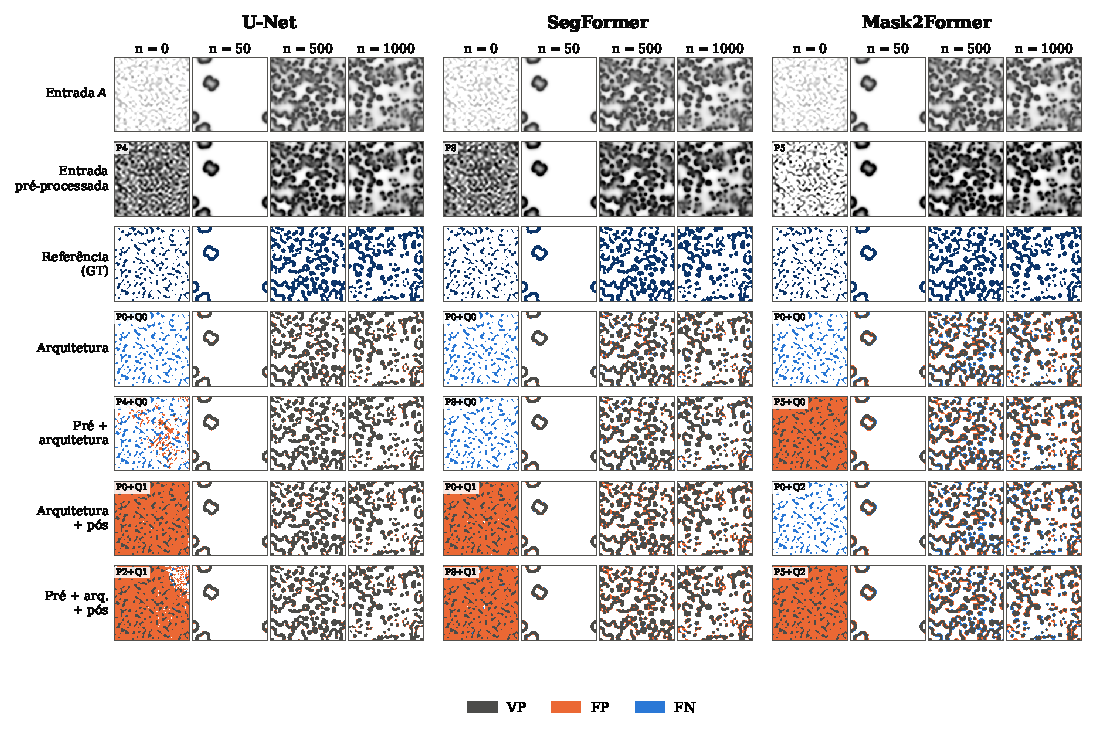
\includegraphics[width=\linewidth]{visual_table_spirals}
\caption{Tabela visual do regime \textit{spirals}. Para cada arquitetura: entrada $A$, entrada pré-processada, referência e máscaras das quatro condições nos instantes 0, 50, 500 e 1000. Cinza-escuro: verdadeiro positivo (VP); laranja: falso positivo; azul: falso negativo. O código da configuração aparece na primeira coluna de cada bloco.}
\label{fig:vt_spirals}
\end{figure}

\begin{figure}[htbp]
\centering
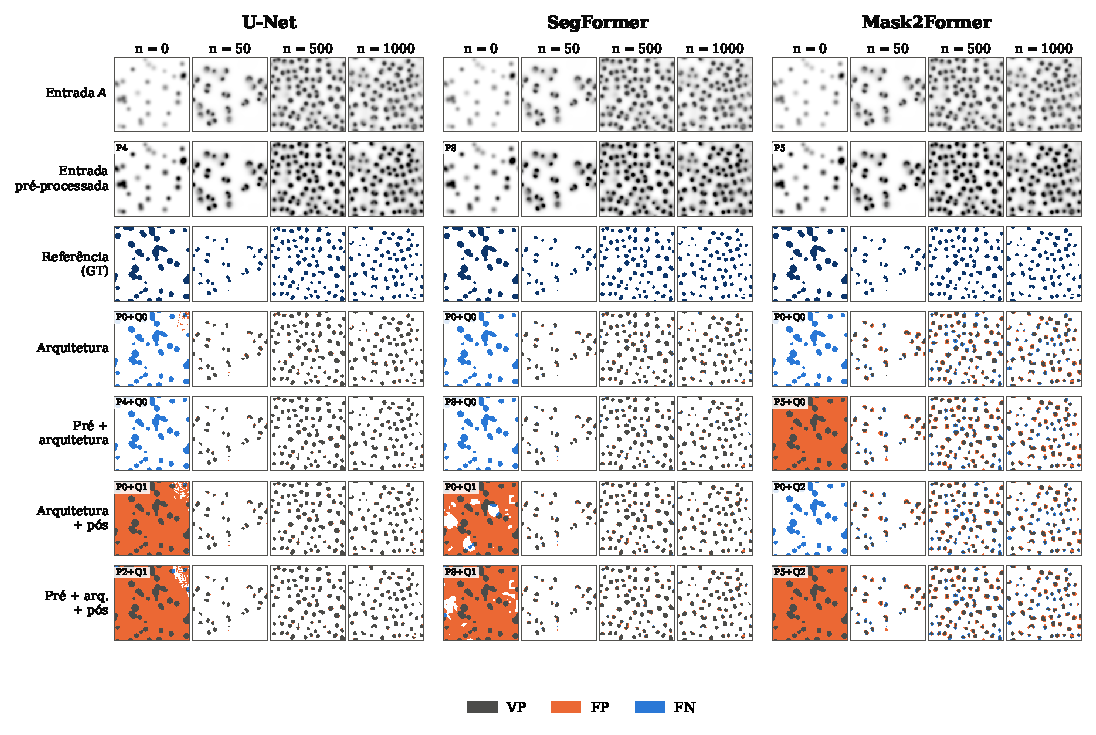
\includegraphics[width=\linewidth]{visual_table_gliders}
\caption{Tabela visual do regime \textit{gliders}, com manchas que se deslocam e se dividem. Mesma organização da Figura~\ref{fig:vt_spirals}.}
\label{fig:vt_gliders}
\end{figure}

\begin{figure}[htbp]
\centering
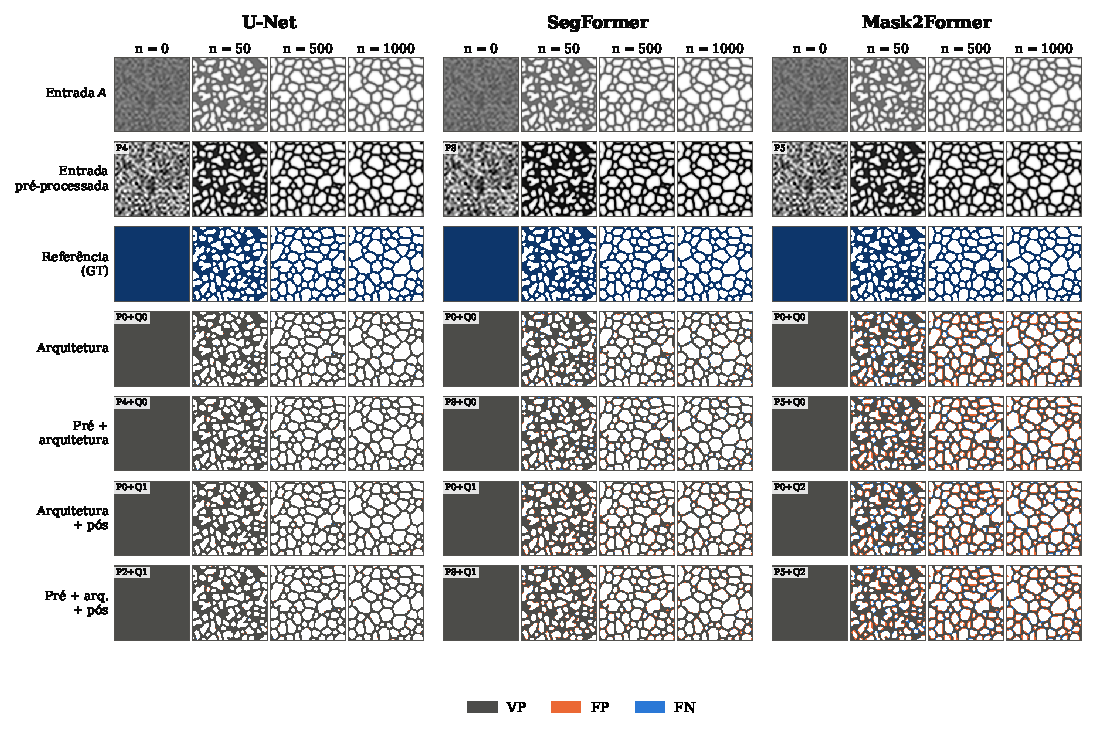
\includegraphics[width=\linewidth]{visual_table_bubbles}
\caption{Tabela visual do regime \textit{bubbles}, com paredes finas entre células amplas. Mesma organização da Figura~\ref{fig:vt_spirals}.}
\label{fig:vt_bubbles}
\end{figure}

Três padrões aparecem nas tabelas visuais. No instante $n=0$, as arquiteturas sem pós-processamento erram a maior parte da referência, com predomínio de falsos negativos, enquanto as configurações com limiar reduzido e o Mask2Former com recorte por percentis segmentam quase todo o domínio, com predomínio de falsos positivos. A partir de $n=50$, a U-Net acompanha as estruturas com poucos erros, enquanto o SegFormer e o Mask2Former apresentam erros concentrados nas fronteiras. No Mask2Former, os erros de fronteira persistem em todas as condições, inclusive nas estruturas finas do regime \textit{bubbles}.

\subsection{Arquiteturas e condições do experimento (PP1)}
\label{subsec:pp1}

A Tabela~\ref{tab:principal} apresenta as métricas de sobreposição das três arquiteturas nas quatro condições, no formato sequencial adotado pela turma, junto com a referência clássica, e a Tabela~\ref{tab:classes} apresenta as métricas por classe das mesmas configurações.

\begin{table}[htbp]
\centering
\caption{Resultados no teste (120 trajetórias, 2.520 quadros) nas quatro condições do experimento. Valores médios por trajetória, com a meia-amplitude do intervalo de confiança de 95\% por \textit{bootstrap} estratificado por regime. O pré e o pós-processamento de cada condição foram escolhidos pelo Dice médio na validação. Latência: rede + pós-processamento por quadro de $128\times128$, lote 1, RTX A5000. Em negrito, o maior valor de cada coluna.}
\label{tab:principal}
\footnotesize\setlength{\tabcolsep}{3pt}
\begin{sbcfitwidth}
\begin{tabular}{lllllccccc}
\toprule
Exp. & Condição & Pré & Arquitetura & Pós & IoU & Dice & Precisão & Revocação & Latência (ms) \\
\midrule
E151 & Arquitetura & P0 & U-Net & Q0 & 0{,}947\,{\scriptsize$\pm$0{,}002} & 0{,}953\,{\scriptsize$\pm$0{,}002} & 0{,}956\,{\scriptsize$\pm$0{,}002} & 0{,}954\,{\scriptsize$\pm$0{,}002} & 5{,}62 \\
E160 & Pré + arquitetura & P4 & U-Net & Q0 & 0{,}949\,{\scriptsize$\pm$0{,}002} & 0{,}955\,{\scriptsize$\pm$0{,}002} & \textbf{0{,}958\,{\scriptsize$\pm$0{,}002}} & 0{,}954\,{\scriptsize$\pm$0{,}002} & 5{,}77 \\
E152 & Arquitetura + pós & P0 & U-Net & Q1 & 0{,}949\,{\scriptsize$\pm$0{,}002} & 0{,}961\,{\scriptsize$\pm$0{,}002} & 0{,}950\,{\scriptsize$\pm$0{,}002} & 0{,}996\,{\scriptsize$\pm$0{,}001} & 5{,}63 \\
E006 & Pré + arquitetura + pós & P2 & U-Net & Q1 & \textbf{0{,}950\,{\scriptsize$\pm$0{,}002}} & \textbf{0{,}962\,{\scriptsize$\pm$0{,}002}} & 0{,}951\,{\scriptsize$\pm$0{,}002} & \textbf{0{,}997\,{\scriptsize$\pm$0{,}000}} & 5{,}70 \\
\midrule
E167 & Arquitetura & P0 & SegFormer & Q0 & 0{,}837\,{\scriptsize$\pm$0{,}004} & 0{,}892\,{\scriptsize$\pm$0{,}003} & 0{,}890\,{\scriptsize$\pm$0{,}003} & 0{,}894\,{\scriptsize$\pm$0{,}003} & 15{,}64 \\
E180 & Pré + arquitetura & P8 & SegFormer & Q0 & 0{,}838\,{\scriptsize$\pm$0{,}004} & 0{,}892\,{\scriptsize$\pm$0{,}003} & 0{,}890\,{\scriptsize$\pm$0{,}003} & 0{,}895\,{\scriptsize$\pm$0{,}003} & 16{,}14 \\
E168 & Arquitetura + pós & P0 & SegFormer & Q1 & 0{,}826\,{\scriptsize$\pm$0{,}005} & 0{,}893\,{\scriptsize$\pm$0{,}003} & 0{,}844\,{\scriptsize$\pm$0{,}004} & 0{,}973\,{\scriptsize$\pm$0{,}001} & 15{,}66 \\
E086 & Pré + arquitetura + pós & P8 & SegFormer & Q1 & 0{,}826\,{\scriptsize$\pm$0{,}005} & 0{,}893\,{\scriptsize$\pm$0{,}003} & 0{,}845\,{\scriptsize$\pm$0{,}004} & 0{,}973\,{\scriptsize$\pm$0{,}001} & 16{,}16 \\
\midrule
E183 & Arquitetura & P0 & Mask2Former & Q0 & 0{,}649\,{\scriptsize$\pm$0{,}014} & 0{,}768\,{\scriptsize$\pm$0{,}009} & 0{,}748\,{\scriptsize$\pm$0{,}009} & 0{,}792\,{\scriptsize$\pm$0{,}009} & 38{,}66 \\
E193 & Pré + arquitetura & P5 & Mask2Former & Q0 & 0{,}659\,{\scriptsize$\pm$0{,}014} & 0{,}782\,{\scriptsize$\pm$0{,}009} & 0{,}739\,{\scriptsize$\pm$0{,}010} & 0{,}857\,{\scriptsize$\pm$0{,}007} & 43{,}46 \\
E185 & Arquitetura + pós & P0 & Mask2Former & Q2 & 0{,}650\,{\scriptsize$\pm$0{,}014} & 0{,}769\,{\scriptsize$\pm$0{,}009} & 0{,}758\,{\scriptsize$\pm$0{,}009} & 0{,}782\,{\scriptsize$\pm$0{,}009} & 39{,}05 \\
E122 & Pré + arquitetura + pós & P5 & Mask2Former & Q2 & 0{,}661\,{\scriptsize$\pm$0{,}014} & 0{,}784\,{\scriptsize$\pm$0{,}009} & 0{,}749\,{\scriptsize$\pm$0{,}010} & 0{,}848\,{\scriptsize$\pm$0{,}008} & 43{,}85 \\
\midrule
REF & Referência clássica & -- & Otsu em $A$ & -- & 0{,}826\,{\scriptsize$\pm$0{,}013} & 0{,}888\,{\scriptsize$\pm$0{,}008} & 0{,}833\,{\scriptsize$\pm$0{,}013} & 0{,}967\,{\scriptsize$\pm$0{,}002} & 0{,}30 \\
\bottomrule
\end{tabular}
\end{sbcfitwidth}
\end{table}


A U-Net obteve Dice de 0,953 sem pré e pós-processamento e de 0,962 na combinação de pré e pós-processamento selecionada (P2+Q1). O SegFormer obteve 0,892 sozinho e entre 0,892 e 0,893 nas condições com processamento, e o Mask2Former, 0,768 sozinho e 0,784 com pré e pós-processamento (P5+Q2). A referência clássica, que apenas limiariza $A$ em cada quadro, alcançou Dice de 0,888, valor cujo intervalo de confiança se sobrepõe ao do SegFormer e que fica acima do Mask2Former em todas as suas condições. A resposta a PP1, considerando todos os instantes, é que a U-Net supera a referência em 6,5 a 7,4 pontos, o SegFormer não se distingue dela, e o Mask2Former fica abaixo dela em 10,5 a 12,0 pontos. A referência clássica apresenta revocação de 0,967 e precisão de 0,833, o que indica que a região de depleção de $A$, mais larga que a estrutura de $B$, produz falsos positivos nas bordas.

\begin{table}[htbp]
\centering
\caption{Métricas por classe no teste para as configurações da Tabela~\ref{tab:principal}: IoU da classe estrutura, IoU e Dice da classe fundo e mIoU, média do IoU das duas classes. Média $\pm$ meia-amplitude do IC de 95\%.}
\label{tab:classes}
\footnotesize\setlength{\tabcolsep}{3pt}
\begin{sbcfitwidth}
\begin{tabular}{lllcccc}
\toprule
Exp. & Arquitetura & Condição & IoU estrutura & IoU fundo & Dice fundo & mIoU \\
\midrule
E151 & U-Net & Arquitetura & 0{,}947\,{\scriptsize$\pm$0{,}002} & 0{,}986\,{\scriptsize$\pm$0{,}001} & 0{,}992\,{\scriptsize$\pm$0{,}001} & 0{,}967\,{\scriptsize$\pm$0{,}001} \\
E160 & U-Net & Pré + arquitetura & 0{,}949\,{\scriptsize$\pm$0{,}002} & 0{,}986\,{\scriptsize$\pm$0{,}001} & 0{,}992\,{\scriptsize$\pm$0{,}001} & 0{,}967\,{\scriptsize$\pm$0{,}001} \\
E152 & U-Net & Arquitetura + pós & 0{,}949\,{\scriptsize$\pm$0{,}002} & 0{,}952\,{\scriptsize$\pm$0{,}002} & 0{,}957\,{\scriptsize$\pm$0{,}002} & 0{,}950\,{\scriptsize$\pm$0{,}002} \\
E006 & U-Net & Pré + arquitetura + pós & 0{,}950\,{\scriptsize$\pm$0{,}002} & 0{,}952\,{\scriptsize$\pm$0{,}002} & 0{,}957\,{\scriptsize$\pm$0{,}002} & 0{,}951\,{\scriptsize$\pm$0{,}002} \\
\midrule
E167 & SegFormer & Arquitetura & 0{,}837\,{\scriptsize$\pm$0{,}004} & 0{,}928\,{\scriptsize$\pm$0{,}002} & 0{,}961\,{\scriptsize$\pm$0{,}001} & 0{,}883\,{\scriptsize$\pm$0{,}003} \\
E180 & SegFormer & Pré + arquitetura & 0{,}838\,{\scriptsize$\pm$0{,}004} & 0{,}929\,{\scriptsize$\pm$0{,}002} & 0{,}962\,{\scriptsize$\pm$0{,}001} & 0{,}883\,{\scriptsize$\pm$0{,}003} \\
E168 & SegFormer & Arquitetura + pós & 0{,}826\,{\scriptsize$\pm$0{,}005} & 0{,}872\,{\scriptsize$\pm$0{,}002} & 0{,}912\,{\scriptsize$\pm$0{,}002} & 0{,}849\,{\scriptsize$\pm$0{,}003} \\
E086 & SegFormer & Pré + arquitetura + pós & 0{,}826\,{\scriptsize$\pm$0{,}005} & 0{,}873\,{\scriptsize$\pm$0{,}002} & 0{,}912\,{\scriptsize$\pm$0{,}002} & 0{,}850\,{\scriptsize$\pm$0{,}003} \\
\midrule
E183 & Mask2Former & Arquitetura & 0{,}649\,{\scriptsize$\pm$0{,}014} & 0{,}836\,{\scriptsize$\pm$0{,}007} & 0{,}908\,{\scriptsize$\pm$0{,}004} & 0{,}742\,{\scriptsize$\pm$0{,}008} \\
E193 & Mask2Former & Pré + arquitetura & 0{,}659\,{\scriptsize$\pm$0{,}014} & 0{,}796\,{\scriptsize$\pm$0{,}006} & 0{,}866\,{\scriptsize$\pm$0{,}003} & 0{,}727\,{\scriptsize$\pm$0{,}008} \\
E185 & Mask2Former & Arquitetura + pós & 0{,}650\,{\scriptsize$\pm$0{,}014} & 0{,}839\,{\scriptsize$\pm$0{,}007} & 0{,}910\,{\scriptsize$\pm$0{,}004} & 0{,}744\,{\scriptsize$\pm$0{,}008} \\
E122 & Mask2Former & Pré + arquitetura + pós & 0{,}661\,{\scriptsize$\pm$0{,}014} & 0{,}800\,{\scriptsize$\pm$0{,}006} & 0{,}869\,{\scriptsize$\pm$0{,}003} & 0{,}730\,{\scriptsize$\pm$0{,}008} \\
\midrule
REF & Otsu em $A$ & -- & 0{,}826\,{\scriptsize$\pm$0{,}013} & 0{,}916\,{\scriptsize$\pm$0{,}005} & 0{,}951\,{\scriptsize$\pm$0{,}003} & 0{,}871\,{\scriptsize$\pm$0{,}008} \\
\bottomrule
\end{tabular}
\end{sbcfitwidth}
\end{table}


As métricas por classe mostram um aspecto que o Dice da classe estrutura não revela. Na U-Net, a otimização do limiar elevou o Dice da estrutura, mas reduziu o IoU da classe fundo de 0,986 para 0,952 e o mIoU de 0,967 para 0,950; no SegFormer, o IoU do fundo caiu de 0,928 para 0,872. A troca decorre do limiar escolhido na validação, 0,2 para a U-Net e para o SegFormer, que amplia a região classificada como estrutura.

\subsection{Efeito do pré-processamento (PP2)}
\label{subsec:pp2}

A Tabela~\ref{tab:efeitos} isola o efeito de cada técnica pela diferença pareada do Dice em relação à arquitetura sozinha. A parte superior corresponde aos pré-processamentos.

\begin{table}[htbp]
\centering
\caption{Efeito de cada técnica isolada: diferença pareada do Dice no teste (em pontos percentuais) em relação à arquitetura sem pré e pós-processamento (P0+Q0), calculada nas mesmas 120 trajetórias, com IC de 95\% por \textit{bootstrap} estratificado por regime. Em negrito, intervalos que não contêm zero; $\blacktriangle$ indica aumento e $\blacktriangledown$, redução do Dice. Valores com duas casas; efeitos com magnitude inferior a 0,005 ponto aparecem como $\pm$0,00, ainda que seu intervalo exclua zero.}
\label{tab:efeitos}
\footnotesize\setlength{\tabcolsep}{3pt}
\begin{sbcfitwidth}
\begin{tabular}{llccc}
\toprule
Código & Técnica & U-Net & SegFormer & Mask2Former \\
\midrule
P1 & Normalização 	extit{z-score} & \textbf{$-$0{,}11 [$-$0{,}15; $-$0{,}07]}$\blacktriangledown$ & \textbf{+0{,}03 [+0{,}03; +0{,}04]}$\blacktriangle$ & \textbf{+0{,}13 [+0{,}11; +0{,}15]}$\blacktriangle$ \\
P2 & Normalização RMS & \textbf{+0{,}15 [+0{,}10; +0{,}19]}$\blacktriangle$ & +0{,}00 [$-$0{,}00; +0{,}01] & \textbf{+0{,}17 [+0{,}14; +0{,}21]}$\blacktriangle$ \\
P3 & Escalonamento robusto & \textbf{$-$0{,}08 [$-$0{,}11; $-$0{,}05]}$\blacktriangledown$ & \textbf{+0{,}03 [+0{,}02; +0{,}04]}$\blacktriangle$ & \textbf{+0{,}05 [+0{,}02; +0{,}08]}$\blacktriangle$ \\
P4 & Normalização mín--máx & \textbf{+0{,}17 [+0{,}10; +0{,}25]}$\blacktriangle$ & $-$0{,}00 [$-$0{,}01; +0{,}00] & +0{,}16 [$-$0{,}06; +0{,}40] \\
P5 & Recorte por percentis & \textbf{$-$0{,}10 [$-$0{,}13; $-$0{,}07]}$\blacktriangledown$ & $-$0{,}00 [$-$0{,}01; +0{,}00] & \textbf{+1{,}37 [+1{,}30; +1{,}45]}$\blacktriangle$ \\
P6 & Suavização gaussiana & \textbf{$-$0{,}09 [$-$0{,}12; $-$0{,}06]}$\blacktriangledown$ & \textbf{$-$0{,}04 [$-$0{,}05; $-$0{,}03]}$\blacktriangledown$ & \textbf{+0{,}55 [+0{,}41; +0{,}68]}$\blacktriangle$ \\
P7 & Filtro de mediana & \textbf{$-$0{,}64 [$-$1{,}07; $-$0{,}31]}$\blacktriangledown$ & $-$0{,}01 [$-$0{,}01; +0{,}00] & \textbf{+0{,}25 [+0{,}17; +0{,}32]}$\blacktriangle$ \\
P8 & Filtro bilateral & \textbf{$-$0{,}15 [$-$0{,}18; $-$0{,}12]}$\blacktriangledown$ & \textbf{+0{,}06 [+0{,}05; +0{,}06]}$\blacktriangle$ & +0{,}00 [$-$0{,}02; +0{,}03] \\
P9 & Difusão anisotrópica & \textbf{$-$0{,}49 [$-$0{,}54; $-$0{,}44]}$\blacktriangledown$ & +0{,}00 [$-$0{,}01; +0{,}02] & \textbf{+0{,}15 [+0{,}13; +0{,}17]}$\blacktriangle$ \\
P10 & Remoção de ruído por 	extit{wavelets} & +0{,}03 [$-$0{,}03; +0{,}08] & \textbf{+0{,}00 [+0{,}00; +0{,}01]}$\blacktriangle$ & \textbf{+0{,}07 [+0{,}04; +0{,}10]}$\blacktriangle$ \\
\midrule
Q1 & Otimização do limiar & \textbf{+0{,}84 [+0{,}76; +0{,}92]}$\blacktriangle$ & +0{,}07 [$-$0{,}03; +0{,}18] & $-$0{,}01 [$-$0{,}04; +0{,}03] \\
Q2 & Abertura morfológica & \textbf{$-$1{,}28 [$-$1{,}46; $-$1{,}11]}$\blacktriangledown$ & \textbf{$-$0{,}25 [$-$0{,}39; $-$0{,}11]}$\blacktriangledown$ & \textbf{+0{,}05 [+0{,}03; +0{,}07]}$\blacktriangle$ \\
Q3 & Fechamento morfológico & \textbf{$-$0{,}18 [$-$0{,}20; $-$0{,}16]}$\blacktriangledown$ & \textbf{+0{,}10 [+0{,}09; +0{,}11]}$\blacktriangle$ & \textbf{$-$0{,}03 [$-$0{,}05; $-$0{,}01]}$\blacktriangledown$ \\
Q4 & Filtragem de componentes conexos & \textbf{$-$0{,}00 [$-$0{,}00; $-$0{,}00]}$\blacktriangledown$ & \textbf{+0{,}00 [+0{,}00; +0{,}00]}$\blacktriangle$ & \textbf{+0{,}00 [+0{,}00; +0{,}00]}$\blacktriangle$ \\
Q5 & Filtragem de consistência temporal & \textbf{$-$11{,}29 [$-$13{,}15; $-$9{,}21]}$\blacktriangledown$ & \textbf{$-$10{,}58 [$-$12{,}37; $-$8{,}59]}$\blacktriangledown$ & \textbf{$-$8{,}63 [$-$10{,}08; $-$7{,}04]}$\blacktriangledown$ \\
\bottomrule
\end{tabular}
\end{sbcfitwidth}
\end{table}


Na U-Net, os efeitos dos pré-processamentos ficaram entre $-0{,}64$ e $+0{,}17$ ponto percentual. Os filtros de mediana ($-0{,}64$) e de difusão anisotrópica ($-0{,}49$) produziram as maiores reduções, e as normalizações RMS ($+0{,}15$) e mín--máx ($+0{,}17$) os maiores aumentos. No SegFormer, todos os efeitos ficaram abaixo de 0,07 ponto em módulo. No Mask2Former, o recorte por percentis (P5) elevou o Dice em 1,37 ponto, e os demais métodos produziram efeitos entre 0,00 e $+0{,}55$ ponto. A remoção de ruído por \textit{wavelets} (P10) teve efeitos entre 0,00 e $+0{,}07$ ponto. A resposta a PP2 é que o pré-processamento produziu alterações pequenas em relação às diferenças entre arquiteturas; o maior efeito, o do recorte por percentis no Mask2Former, é examinado na Seção~\ref{subsec:sensibilidade}.

\subsection{Efeito do pós-processamento (PP3)}
\label{subsec:pp3}

A parte inferior da Tabela~\ref{tab:efeitos} mostra que a otimização do limiar (Q1) elevou o Dice da U-Net em 0,84 ponto, sem efeito distinguível de zero no SegFormer e no Mask2Former. A abertura morfológica (Q2) reduziu o Dice da U-Net em 1,28 ponto e o do SegFormer em 0,25 ponto, e elevou o do Mask2Former em 0,05 ponto. O fechamento (Q3) reduziu o Dice da U-Net em 0,18 ponto e elevou o do SegFormer em 0,10 ponto. A filtragem de componentes conexos (Q4) teve efeitos inferiores a 0,005 ponto em módulo, pois as áreas mínimas escolhidas na validação, de 2 a 8 pixels, quase não removeram regiões. A filtragem de consistência temporal (Q5) reduziu o Dice das três arquiteturas em 11,29, 10,58 e 8,63 pontos.

A análise por regime detalha o maior efeito. Na U-Net, a redução causada pelo filtro temporal foi de 31,43 pontos em \textit{gliders} e 28,95 pontos em \textit{spirals}, regimes em que as estruturas se deslocam, contra 0,51 ponto em \textit{bubbles} e 0,33 ponto em \textit{worms}, cujos padrões se estabilizam. A resposta a PP3 é que, entre as técnicas do protocolo, apenas a otimização do limiar elevou o Dice médio de forma apreciável, e apenas na U-Net, enquanto o filtro temporal o reduziu fortemente nos regimes dinâmicos. A Figura~\ref{fig:heat} apresenta o Dice de todas as combinações.

\begin{figure}[htbp]
\centering
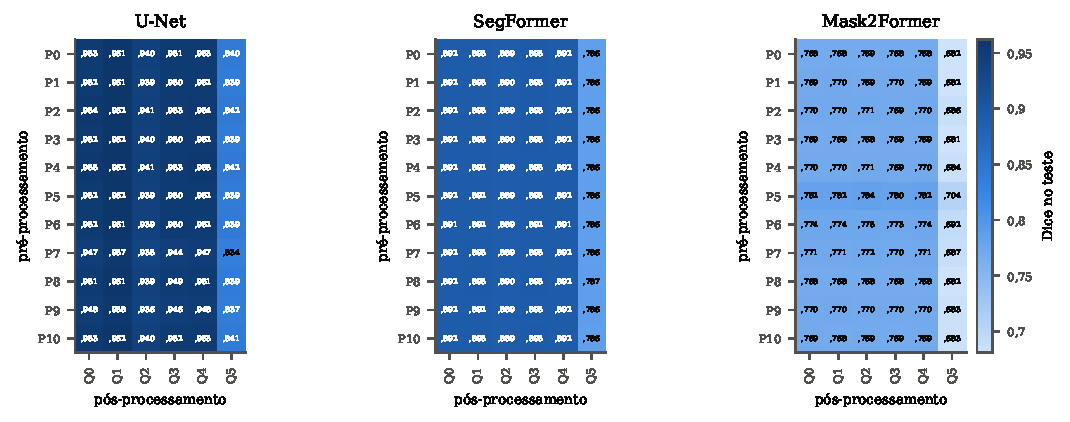
\includegraphics[width=\linewidth]{heatmap_dice}
\caption{Dice no teste de todas as combinações de pré-processamento (linhas) e pós-processamento (colunas) para cada arquitetura, com o zero à esquerda da vírgula omitido. P0 e Q0 indicam os \textit{baselines}.}
\label{fig:heat}
\end{figure}

\subsection{Sensibilidade ao instante inicial}
\label{subsec:sensibilidade}

O instante $n=0$ é um dos 21 instantes amostrados, e nele a condição inicial é aleatória. A Tabela~\ref{tab:sensibilidade} separa o Dice desse instante do Dice dos demais.

\begin{table}[htbp]
\centering
\caption{Sensibilidade ao instante inicial: Dice médio no teste em todos os 21 instantes, apenas em $n=0$ e nos 20 instantes $n\geq50$, para as configurações selecionadas na validação. Média por trajetória, com IC de 95\% por \textit{bootstrap} estratificado por regime para $n\geq50$.}
\label{tab:sensibilidade}
\footnotesize\setlength{\tabcolsep}{3pt}
\begin{sbcfitwidth}
\begin{tabular}{lllccc}
\toprule
Exp. & Arquitetura & Condição & Dice (todos) & Dice ($n=0$) & Dice ($n\geq50$) \\
\midrule
E151 & U-Net & Arquitetura & 0{,}953 & 0{,}120 & 0{,}995\,{\scriptsize$\pm$0{,}001} \\
E160 & U-Net & Pré + arquitetura & 0{,}955 & 0{,}153 & 0{,}995\,{\scriptsize$\pm$0{,}001} \\
E152 & U-Net & Arquitetura + pós & 0{,}961 & 0{,}353 & 0{,}992\,{\scriptsize$\pm$0{,}001} \\
E006 & U-Net & Pré + arquitetura + pós & 0{,}962 & 0{,}354 & 0{,}992\,{\scriptsize$\pm$0{,}001} \\
\midrule
E167 & SegFormer & Arquitetura & 0{,}892 & 0{,}100 & 0{,}931\,{\scriptsize$\pm$0{,}002} \\
E180 & SegFormer & Pré + arquitetura & 0{,}892 & 0{,}100 & 0{,}932\,{\scriptsize$\pm$0{,}002} \\
E168 & SegFormer & Arquitetura + pós & 0{,}893 & 0{,}357 & 0{,}919\,{\scriptsize$\pm$0{,}003} \\
E086 & SegFormer & Pré + arquitetura + pós & 0{,}893 & 0{,}357 & 0{,}920\,{\scriptsize$\pm$0{,}003} \\
\midrule
E183 & Mask2Former & Arquitetura & 0{,}768 & 0{,}102 & 0{,}801\,{\scriptsize$\pm$0{,}009} \\
E193 & Mask2Former & Pré + arquitetura & 0{,}782 & 0{,}353 & 0{,}803\,{\scriptsize$\pm$0{,}009} \\
E185 & Mask2Former & Arquitetura + pós & 0{,}769 & 0{,}101 & 0{,}802\,{\scriptsize$\pm$0{,}009} \\
E122 & Mask2Former & Pré + arquitetura + pós & 0{,}784 & 0{,}353 & 0{,}805\,{\scriptsize$\pm$0{,}009} \\
\midrule
REF & Otsu em $A$ & Referência clássica & 0{,}888 & 0{,}241 & 0{,}921\,{\scriptsize$\pm$0{,}008} \\
\bottomrule
\end{tabular}
\end{sbcfitwidth}
\end{table}


As arquiteturas sem pós-processamento obtiveram Dice entre 0,100 e 0,120 em $n=0$, com área prevista de cerca de 11\% do domínio na U-Net, contra 25,3\% da referência. Com o limiar de 0,2, a U-Net passou a segmentar 95,2\% do domínio nesse instante, e o Dice de $n=0$ subiu para 0,353. Nos instantes $n\geq50$, contudo, a configuração P2+Q1 obteve 0,992, abaixo dos 0,995 da U-Net sozinha. Recalculadas sem o instante inicial, as diferenças pareadas mudaram de sinal para a otimização do limiar: $-0{,}28$ ponto na U-Net e $-1{,}21$ ponto no SegFormer, ambas distinguíveis de zero. O efeito do recorte por percentis no Mask2Former caiu de 1,37 para 0,18 ponto, pois nessa configuração a área prevista em $n=0$ também chegou a 99,2\% do domínio. Os efeitos da abertura morfológica e do filtro temporal mantiveram o sinal e a magnitude. Sem o instante inicial, o SegFormer obteve Dice de 0,931, acima dos 0,921 da referência clássica.

\subsection{Evolução temporal das estruturas (PP4)}
\label{subsec:pp4}

A Tabela~\ref{tab:temporal} apresenta as métricas temporais, e a Figura~\ref{fig:temporal} mostra o Dice e a área segmentada ao longo dos instantes.

\begin{table}[htbp]
\centering
\caption{Métricas temporais no teste para as configurações da Tabela~\ref{tab:principal}. AVE: erro de variação de área (\% do domínio por instante amostrado); CDE: erro de deslocamento dos centroides das estruturas (px, distância periódica); TC: consistência temporal das máscaras, com o valor do GT na última linha; TCE $=|TC_{pred}-TC_{GT}|$. Média $\pm$ meia-amplitude do IC de 95\%.}
\label{tab:temporal}
\footnotesize\setlength{\tabcolsep}{3pt}
\begin{sbcfitwidth}
\begin{tabular}{lllcccc}
\toprule
Exp. & Arquitetura & Condição & AVE (\%) & CDE (px) & TC & TCE \\
\midrule
E151 & U-Net & Arquitetura & 0{,}764\,{\scriptsize$\pm$0{,}050} & 2{,}68\,{\scriptsize$\pm$0{,}34} & 0{,}686 & 0{,}010\,{\scriptsize$\pm$0{,}002} \\
E160 & U-Net & Pré + arquitetura & 0{,}593\,{\scriptsize$\pm$0{,}068} & 2{,}16\,{\scriptsize$\pm$0{,}34} & 0{,}683 & 0{,}007\,{\scriptsize$\pm$0{,}001} \\
E152 & U-Net & Arquitetura + pós & 3{,}554\,{\scriptsize$\pm$0{,}142} & 1{,}57\,{\scriptsize$\pm$0{,}22} & 0{,}691 & 0{,}009\,{\scriptsize$\pm$0{,}001} \\
E006 & U-Net & Pré + arquitetura + pós & 3{,}579\,{\scriptsize$\pm$0{,}148} & 1{,}42\,{\scriptsize$\pm$0{,}21} & 0{,}691 & 0{,}008\,{\scriptsize$\pm$0{,}001} \\
\midrule
E167 & SegFormer & Arquitetura & 0{,}892\,{\scriptsize$\pm$0{,}049} & 7{,}16\,{\scriptsize$\pm$0{,}69} & 0{,}685 & 0{,}013\,{\scriptsize$\pm$0{,}002} \\
E180 & SegFormer & Pré + arquitetura & 0{,}891\,{\scriptsize$\pm$0{,}050} & 7{,}18\,{\scriptsize$\pm$0{,}67} & 0{,}685 & 0{,}013\,{\scriptsize$\pm$0{,}002} \\
E168 & SegFormer & Arquitetura + pós & 3{,}870\,{\scriptsize$\pm$0{,}147} & 7{,}85\,{\scriptsize$\pm$0{,}62} & 0{,}698 & 0{,}014\,{\scriptsize$\pm$0{,}001} \\
E086 & SegFormer & Pré + arquitetura + pós & 3{,}868\,{\scriptsize$\pm$0{,}148} & 7{,}91\,{\scriptsize$\pm$0{,}60} & 0{,}697 & 0{,}014\,{\scriptsize$\pm$0{,}001} \\
\midrule
E183 & Mask2Former & Arquitetura & 1{,}203\,{\scriptsize$\pm$0{,}055} & 9{,}47\,{\scriptsize$\pm$0{,}64} & 0{,}686 & 0{,}014\,{\scriptsize$\pm$0{,}002} \\
E193 & Mask2Former & Pré + arquitetura & 4{,}083\,{\scriptsize$\pm$0{,}142} & 7{,}13\,{\scriptsize$\pm$0{,}65} & 0{,}697 & 0{,}012\,{\scriptsize$\pm$0{,}001} \\
E185 & Mask2Former & Arquitetura + pós & 1{,}196\,{\scriptsize$\pm$0{,}055} & 9{,}95\,{\scriptsize$\pm$0{,}76} & 0{,}684 & 0{,}015\,{\scriptsize$\pm$0{,}002} \\
E122 & Mask2Former & Pré + arquitetura + pós & 4{,}104\,{\scriptsize$\pm$0{,}141} & 7{,}45\,{\scriptsize$\pm$0{,}81} & 0{,}695 & 0{,}010\,{\scriptsize$\pm$0{,}001} \\
\midrule
REF & Otsu em $A$ & -- & 1{,}761\,{\scriptsize$\pm$0{,}127} & 3{,}17\,{\scriptsize$\pm$0{,}43} & 0{,}710 & 0{,}027\,{\scriptsize$\pm$0{,}003} \\
GT & Referência & -- & -- & -- & 0{,}689 & -- \\
\bottomrule
\end{tabular}
\end{sbcfitwidth}
\end{table}


\begin{figure}[htbp]
\centering
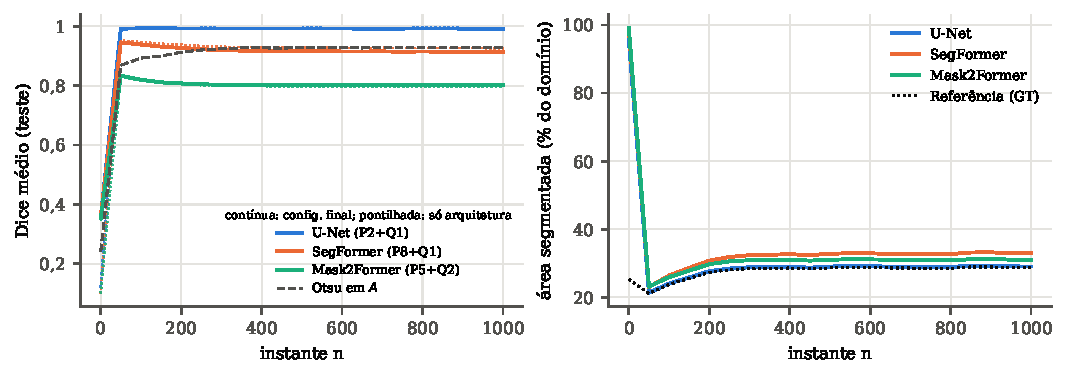
\includegraphics[width=\linewidth]{temporal_dice_area}
\caption{Dice médio no teste por instante (esquerda) para a configuração final de cada arquitetura (linha contínua), para a arquitetura sozinha (pontilhada) e para Otsu em $A$ (tracejada), e área segmentada média, em percentual do domínio (direita).}
\label{fig:temporal}
\end{figure}

Em $n=50$, a U-Net sozinha já alcançava Dice de 0,994, o SegFormer 0,952 e o Mask2Former 0,829, e a partir de $n=100$ os valores médios foram de 0,995, 0,930 e 0,800. A referência clássica obteve 0,869 em $n=50$ e 0,923 a partir de $n=100$. A U-Net sozinha teve o menor erro de variação de área, 0,76\% do domínio por instante, e TCE de 0,010, para uma consistência temporal de 0,689 na referência. A configuração final da U-Net (P2+Q1) reduziu o erro de posição de 2,68 para 1,42 pixel, mas elevou o erro de variação de área para 3,58\%, efeito do salto de área entre o instante inicial superestimado e os instantes seguintes. O SegFormer e o Mask2Former mantiveram erros de posição de 7,1 a 10,0 pixels. A resposta a PP4 é que a U-Net acompanhou a evolução das estruturas a partir do primeiro instante amostrado após a condição inicial, enquanto nenhuma configuração segmentou o instante inicial de forma informativa.

\subsection{Regimes e custo computacional}
\label{subsec:regimes-custo}

A Tabela~\ref{tab:regime} apresenta o Dice por regime.

\begin{table}[htbp]
\centering
\caption{Dice no teste por regime para cada arquitetura sozinha (P0+Q0), para a configuração final de cada arquitetura (pré + arquitetura + pós) e para a referência clássica. Vinte trajetórias por regime.}
\label{tab:regime}
\footnotesize\setlength{\tabcolsep}{3pt}
\begin{sbcfitwidth}
\begin{tabular}{lcccccc}
\toprule
Configuração & Gliders & Bubbles & Maze & Worms & Spirals & Spots \\
\midrule
E151 U-Net (P0+Q0) & 0{,}948 & 0{,}979 & 0{,}950 & 0{,}948 & 0{,}943 & 0{,}949 \\
E006 U-Net (P2+Q1) & 0{,}963 & 0{,}981 & 0{,}959 & 0{,}956 & 0{,}955 & 0{,}958 \\
E167 SegFormer (P0+Q0) & 0{,}927 & 0{,}952 & 0{,}865 & 0{,}868 & 0{,}905 & 0{,}833 \\
E086 SegFormer (P8+Q1) & 0{,}941 & 0{,}952 & 0{,}859 & 0{,}866 & 0{,}912 & 0{,}829 \\
E183 Mask2Former (P0+Q0) & 0{,}833 & 0{,}800 & 0{,}781 & 0{,}712 & 0{,}816 & 0{,}667 \\
E122 Mask2Former (P5+Q2) & 0{,}850 & 0{,}803 & 0{,}795 & 0{,}726 & 0{,}835 & 0{,}692 \\
\midrule
REF Otsu em $A$ & 0{,}852 & 0{,}917 & 0{,}938 & 0{,}896 & 0{,}821 & 0{,}906 \\
\bottomrule
\end{tabular}
\end{sbcfitwidth}
\end{table}


A U-Net sozinha manteve Dice entre 0,943 e 0,979 em todos os regimes. O SegFormer obteve seus menores valores em \textit{spots} (0,833), \textit{maze} (0,865) e \textit{worms} (0,868), abaixo dos 0,906, 0,938 e 0,896 da referência clássica nesses regimes, e o Mask2Former também obteve seu menor valor em \textit{spots} (0,667). A Tabela~\ref{tab:custo} resume o custo das arquiteturas.

\begin{table}[htbp]
\centering
\caption{Tamanho e custo das arquiteturas na entrada de referência (P0): parâmetros, tempo de treino de 20 épocas com até cinco treinos simultâneos na mesma GPU, época selecionada na validação, memória máxima de GPU no treino (lote 32) e na inferência (lote 1), latência (lote 1) e vazão (lote 32), estas medidas com a GPU dedicada. NVIDIA RTX A5000.}
\label{tab:custo}
\footnotesize\setlength{\tabcolsep}{3pt}
\begin{sbcfitwidth}
\begin{tabular}{lccccccc}
\toprule
Arquitetura & Parâm. (M) & Treino (min) & Época & Mem. treino (MiB) & Mem. inf. (MiB) & Latência (ms) & Vazão (quadros/s) \\
\midrule
U-Net & 24{,}4 & 20{,}5 & 20/20 & 878 & 170 & 5{,}58 & 4932 \\
SegFormer & 27{,}3 & 34{,}6 & 20/20 & 2376 & 227 & 15{,}61 & 2073 \\
Mask2Former & 47{,}4 & 272{,}6 & 2/20 & 4526 & 287 & 38{,}63 & 552 \\
\bottomrule
\end{tabular}
\end{sbcfitwidth}
\end{table}


A U-Net teve a menor latência (5,58 ms) e o menor tempo de treino, enquanto o Mask2Former, com 47,4 milhões de parâmetros, teve latência de 38,63 ms e o maior tempo de treino nas condições de execução compartilhada. A época selecionada também diferiu entre as arquiteturas: no SegFormer, a melhor época foi a 19 ou a 20 em todas as entradas, o que indica que o Dice de validação ainda crescia ao fim do orçamento; no Mask2Former, ficou entre a primeira e a nona época, pois seu Dice de validação permaneceu entre 0,771 e 0,776 ao longo das 20 épocas na entrada de referência (Figura~\ref{fig:treino}).

\begin{figure}[htbp]
\centering
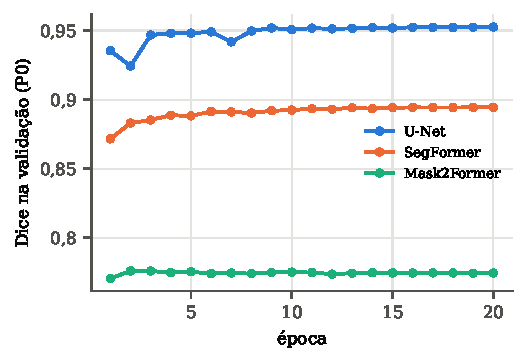
\includegraphics[width=0.6\linewidth]{training_curves}
\caption{Dice na validação ao longo das 20 épocas de treino, na entrada de referência (P0).}
\label{fig:treino}
\end{figure}

%% =====================================================================
\section{Discussão}
\label{sec:discussao}

O principal resultado é que a ordem entre as arquiteturas foi determinada por uma propriedade de projeto, a resolução da saída, mais do que pelas técnicas aplicadas antes ou depois da rede. A U-Net prevê na resolução da entrada, com conexões de salto a partir do estágio de maior resolução, ao passo que o SegFormer e o Mask2Former preveem em $32\times32$ células para uma entrada de $128\times128$. Com estruturas de poucos pixels de diâmetro, uma célula da saída dessas duas arquiteturas cobre parte considerável de uma estrutura, e a fronteira passa a depender da interpolação dos \textit{logits}. Essa interpretação é compatível com a queda do SegFormer nos regimes de menor comprimento de onda, nos quais ficou abaixo da limiarização de $A$. O desenho, contudo, não isola a resolução de saída de outras diferenças entre as arquiteturas, como o \textit{backbone} e o pré-treinamento.

O efeito pequeno do pré-processamento decorre das propriedades dos dados. Os campos simulados não contêm ruído de aquisição, de modo que os filtros de remoção de ruído têm pouco a remover, enquanto os filtros de suavização removem sinal: a suavização gaussiana atenua os harmônicos que definem fronteiras nítidas, e o filtro de mediana arredonda cantos e remove ligações de um pixel. Essa perda de detalhe é compatível com as reduções observadas na U-Net, a única arquitetura capaz de explorar esse detalhe. As normalizações são, em primeira ordem, transformações afins, cujo efeito tende a ser absorvido pelas camadas de normalização das redes, o que é coerente com efeitos próximos de zero.

A sensibilidade ao instante inicial é o resultado de maior consequência metodológica. Em $n=0$, a condição inicial é aleatória e o campo $A$ ainda não reflete a estrutura de $B$, de modo que nenhuma configuração segmentou esse instante de forma informativa. Ainda assim, um único instante entre 21 bastou para decidir a seleção na validação: um limiar baixo leva a rede a segmentar quase todo o domínio em $n=0$, o que aumenta o Dice desse instante sem nenhuma informação física, e o mesmo efeito explica a maior parte do ganho do recorte por percentis no Mask2Former. Nos instantes com padrão, a otimização do limiar reduziu o Dice da U-Net e do SegFormer e reduziu o IoU da classe fundo, o que mostra que o Dice médio da classe estrutura, usado como critério único de seleção, favoreceu a supersegmentação de um quadro sem informação. A escolha de uma configuração para acompanhar a evolução das estruturas deve, portanto, considerar as métricas por classe e as temporais e excluir ou ponderar o instante inicial quando a condição inicial é aleatória.

Os efeitos do pós-processamento acompanharam a escala das operações em relação às estruturas e à amostragem temporal. A abertura morfológica com disco de raio 1 remove estruturas com menos de três pixels de largura, como as manchas nascentes e as paredes finas do regime \textit{bubbles}, o que explica as reduções na U-Net, cuja predição já preservava esses detalhes. A filtragem de componentes conexos não alterou os resultados porque as redes, aplicadas a campos suaves, quase não produzem regiões isoladas de poucos pixels, de modo que a hipótese de ruído pontual que justifica o método não se verificou neste conjunto. O filtro temporal combina instantes separados por 50 passos amostrados, ou 500 unidades de tempo; nos regimes em que o padrão se desloca, as estruturas mudam de posição nesse intervalo, e a mediana produz máscaras defasadas que apagam mudanças físicas reais, o que é coerente com perdas de cerca de 30 pontos em \textit{gliders} e \textit{spirals} e com a ressalva do próprio protocolo sobre esse método.

O desempenho do Mask2Former deve ser lido com cautela. Seu Dice de validação estabilizou-se nas primeiras épocas e não variou nas seguintes, embora a perda de treino continuasse diminuindo. Esse comportamento é compatível com duas hipóteses não separadas pelo desenho: a limitação da saída em baixa resolução e o treino sem supervisão profunda, que integra a receita original da arquitetura \cite{cheng2022mask2former}. A formulação por classificação de máscaras também foi concebida para objetos e regiões de cenas naturais, e aqui uma única classe se distribui em dezenas de componentes desconexos que precisam ser representados por poucas consultas. Os resultados do Mask2Former caracterizam, assim, a configuração efetivamente treinada, e não o potencial da arquitetura sob a receita original. No SegFormer, a melhor época ao fim do orçamento indica que o limite de 20 épocas do protocolo pode ter restringido seu desempenho.

%% =====================================================================
\section{Limitações}
\label{sec:limitacoes}

Quanto à validade interna, cada configuração foi treinada com uma única semente, e os intervalos de confiança capturam a variação entre trajetórias de teste, mas não entre treinos. O Mask2Former foi treinado sem supervisão profunda, e as arquiteturas diferem simultaneamente em resolução de saída, \textit{backbone} e pré-treinamento, de modo que nenhuma comparação entre elas identifica a causa das diferenças. A seleção das condições pelo Dice médio na validação foi sensível ao instante inicial, como discutido na Seção~\ref{sec:discussao}. Os treinos compartilharam a GPU, o que afeta os tempos de treino reportados, embora não as latências, medidas com a GPU dedicada.

Quanto à validade de construção, a referência foi definida por limiarização de $B$, e não por anotação especialista, e depende da escolha do instante de referência e do critério de Otsu; o experimento mede a recuperação de uma segmentação definida por um critério físico, e não a descoberta de estruturas desconhecidas. A forte anticorrelação entre $A$ e $B$ torna a tarefa mais simples que a segmentação de imagens naturais, razão pela qual a referência clássica foi incluída. O intervalo de 50 instantes entre quadros amostrados limita a resolução temporal das métricas de evolução e penaliza o filtro temporal nos regimes dinâmicos.

Quanto à validade externa, os resultados referem-se a um sistema físico, a 21 instantes por trajetória, a uma GPU e às bibliotecas utilizadas. As redes processam os quadros de forma independente, e apenas o filtro temporal usa contexto entre instantes.

%% =====================================================================
\section{Conclusão}
\label{sec:conclusao}

Este trabalho avaliou o efeito do pré-processamento, da arquitetura e do pós-processamento sobre a segmentação temporal das regiões de reação ativa no sistema de Gray--Scott do The Well, sob o protocolo comum da turma, nas 150 combinações da matriz e em suas linhas de \textit{baseline}, com as 1.200 trajetórias do conjunto. Quanto a PP1, a U-Net obteve Dice de 0,953 sem pré e pós-processamento, acima da referência clássica de Otsu em $A$ (0,888), enquanto o SegFormer não se distinguiu dessa referência (0,892) e o Mask2Former ficou abaixo dela (0,768). Quanto a PP2, o pré-processamento alterou o Dice em no máximo 1,37 ponto percentual, e o maior efeito decorreu do instante inicial.

Quanto a PP3, a otimização do limiar elevou o Dice médio da U-Net em 0,84 ponto, mas passou a reduzi-lo quando o instante inicial foi excluído, e a filtragem de consistência temporal reduziu o Dice de todas as arquiteturas em 8,6 a 11,3 pontos, com perdas de cerca de 30 pontos nos regimes cujas estruturas se deslocam. Quanto a PP4, a U-Net acompanhou a evolução das estruturas a partir do primeiro instante amostrado, com Dice médio de 0,995 a partir de $n=100$, mas nenhuma configuração segmentou o instante inicial aleatório. Nesse conjunto, portanto, a resolução de saída da arquitetura pesou mais que as técnicas aplicadas antes e depois dela, e a seleção de configurações pelo Dice médio mostrou-se sensível a um único instante sem informação física.

A continuidade deste estudo requer repetir os treinos com mais sementes, treinar o Mask2Former com supervisão profunda e variar a resolução de saída das arquiteturas Transformer para separar seu efeito das demais diferenças. Também requer definir o critério de seleção com o instante inicial excluído ou ponderado, avaliar arquiteturas que usem contexto temporal, examinar a sensibilidade da referência ao instante escolhido e integrar estes resultados aos dos demais sistemas físicos da turma no artigo conjunto.

\nocite{turing1952}
\bibliographystyle{sbc}
\bibliography{referencias}

\clearpage
\appendix
\section{Tabela sequencial de todas as combinações}
\label{ap:sequencial}

\begingroup\footnotesize
\setlength{\tabcolsep}{3.2pt}
\begin{longtable}{lllllccccccc}
\caption{Resultados sequenciais e padronizados de todas as combinações no teste. E001--E150: P1--P10 $\times$ arquitetura $\times$ Q1--Q5, matriz do protocolo da turma; E151--E198: linhas de \textit{baseline} sem pré e/ou sem pós-processamento; REF: Otsu em $A$. AVE em \% do domínio, CDE em px e latência em ms por quadro.}\label{tab:sequencial}\\
\toprule
Exp. & Pré & Arquitetura & Pós & IoU & Dice & Prec. & Rev. & AVE & CDE & TCE & Lat. \\
\midrule
\endfirsthead
\toprule
Exp. & Pré & Arquitetura & Pós & IoU & Dice & Prec. & Rev. & AVE & CDE & TCE & Lat. \\
\midrule
\endhead
\bottomrule
\endfoot
E001 & P1 & U-Net & Q1 & 0{,}9488 & 0{,}9615 & 0{,}9504 & 0{,}9979 & 3{,}744 & 1{,}68 & 0{,}0084 & 6{,}09 \\
E002 & P1 & U-Net & Q2 & 0{,}9225 & 0{,}9393 & 0{,}9526 & 0{,}9273 & 0{,}836 & 4{,}65 & 0{,}0135 & 6{,}47 \\
E003 & P1 & U-Net & Q3 & 0{,}9429 & 0{,}9499 & 0{,}9493 & 0{,}9529 & 0{,}842 & 4{,}54 & 0{,}0106 & 6{,}51 \\
E004 & P1 & U-Net & Q4 & 0{,}9467 & 0{,}9519 & 0{,}9535 & 0{,}9525 & 0{,}820 & 4{,}03 & 0{,}0112 & 6{,}41 \\
E005 & P1 & U-Net & Q5 & 0{,}7942 & 0{,}8387 & 0{,}8916 & 0{,}8147 & 1{,}347 & 5{,}81 & 0{,}0720 & 6{,}46 \\
E006 & P2 & U-Net & Q1 & 0{,}9500 & 0{,}9620 & 0{,}9513 & 0{,}9967 & 3{,}579 & 1{,}42 & 0{,}0084 & 5{,}70 \\
E007 & P2 & U-Net & Q2 & 0{,}9237 & 0{,}9409 & 0{,}9585 & 0{,}9285 & 0{,}742 & 2{,}06 & 0{,}0091 & 6{,}09 \\
E008 & P2 & U-Net & Q3 & 0{,}9447 & 0{,}9528 & 0{,}9542 & 0{,}9551 & 0{,}647 & 2{,}28 & 0{,}0066 & 6{,}11 \\
E009 & P2 & U-Net & Q4 & 0{,}9484 & 0{,}9543 & 0{,}9583 & 0{,}9543 & 0{,}666 & 1{,}58 & 0{,}0067 & 6{,}02 \\
E010 & P2 & U-Net & Q5 & 0{,}7961 & 0{,}8418 & 0{,}8947 & 0{,}8170 & 1{,}225 & 3{,}30 & 0{,}0666 & 6{,}06 \\
E011 & P3 & U-Net & Q1 & 0{,}9496 & 0{,}9618 & 0{,}9507 & 0{,}9981 & 3{,}715 & 1{,}78 & 0{,}0084 & 6{,}34 \\
E012 & P3 & U-Net & Q2 & 0{,}9231 & 0{,}9396 & 0{,}9520 & 0{,}9279 & 0{,}830 & 4{,}78 & 0{,}0134 & 6{,}76 \\
E013 & P3 & U-Net & Q3 & 0{,}9433 & 0{,}9502 & 0{,}9481 & 0{,}9534 & 0{,}841 & 4{,}80 & 0{,}0111 & 6{,}75 \\
E014 & P3 & U-Net & Q4 & 0{,}9472 & 0{,}9521 & 0{,}9524 & 0{,}9531 & 0{,}816 & 4{,}18 & 0{,}0112 & 6{,}65 \\
E015 & P3 & U-Net & Q5 & 0{,}7946 & 0{,}8390 & 0{,}8907 & 0{,}8150 & 1{,}347 & 6{,}10 & 0{,}0728 & 6{,}69 \\
E016 & P4 & U-Net & Q1 & 0{,}9502 & 0{,}9620 & 0{,}9518 & 0{,}9928 & 3{,}176 & 1{,}46 & 0{,}0081 & 5{,}78 \\
E017 & P4 & U-Net & Q2 & 0{,}9236 & 0{,}9409 & 0{,}9567 & 0{,}9281 & 0{,}728 & 2{,}92 & 0{,}0093 & 6{,}19 \\
E018 & P4 & U-Net & Q3 & 0{,}9450 & 0{,}9531 & 0{,}9534 & 0{,}9553 & 0{,}588 & 2{,}76 & 0{,}0064 & 6{,}21 \\
E019 & P4 & U-Net & Q4 & 0{,}9485 & 0{,}9546 & 0{,}9574 & 0{,}9544 & 0{,}601 & 2{,}22 & 0{,}0067 & 6{,}10 \\
E020 & P4 & U-Net & Q5 & 0{,}7960 & 0{,}8419 & 0{,}8948 & 0{,}8171 & 1{,}201 & 3{,}86 & 0{,}0662 & 6{,}17 \\
E021 & P5 & U-Net & Q1 & 0{,}9490 & 0{,}9616 & 0{,}9502 & 0{,}9986 & 3{,}761 & 1{,}85 & 0{,}0086 & 5{,}55 \\
E022 & P5 & U-Net & Q2 & 0{,}9228 & 0{,}9395 & 0{,}9517 & 0{,}9280 & 0{,}830 & 4{,}78 & 0{,}0133 & 5{,}94 \\
E023 & P5 & U-Net & Q3 & 0{,}9429 & 0{,}9499 & 0{,}9470 & 0{,}9534 & 0{,}842 & 4{,}85 & 0{,}0107 & 5{,}96 \\
E024 & P5 & U-Net & Q4 & 0{,}9468 & 0{,}9519 & 0{,}9509 & 0{,}9530 & 0{,}817 & 4{,}37 & 0{,}0112 & 5{,}86 \\
E025 & P5 & U-Net & Q5 & 0{,}7945 & 0{,}8390 & 0{,}8897 & 0{,}8151 & 1{,}348 & 6{,}15 & 0{,}0717 & 5{,}93 \\
E026 & P6 & U-Net & Q1 & 0{,}9472 & 0{,}9605 & 0{,}9487 & 0{,}9948 & 3{,}414 & 1{,}57 & 0{,}0085 & 5{,}47 \\
E027 & P6 & U-Net & Q2 & 0{,}9220 & 0{,}9391 & 0{,}9587 & 0{,}9276 & 0{,}831 & 2{,}14 & 0{,}0096 & 5{,}84 \\
E028 & P6 & U-Net & Q3 & 0{,}9423 & 0{,}9503 & 0{,}9546 & 0{,}9534 & 0{,}805 & 2{,}38 & 0{,}0071 & 5{,}88 \\
E029 & P6 & U-Net & Q4 & 0{,}9460 & 0{,}9520 & 0{,}9589 & 0{,}9529 & 0{,}791 & 1{,}68 & 0{,}0073 & 5{,}77 \\
E030 & P6 & U-Net & Q5 & 0{,}7940 & 0{,}8393 & 0{,}8961 & 0{,}8153 & 1{,}323 & 3{,}46 & 0{,}0659 & 5{,}81 \\
E031 & P7 & U-Net & Q1 & 0{,}9403 & 0{,}9566 & 0{,}9432 & 0{,}9962 & 3{,}765 & 2{,}01 & 0{,}0094 & 6{,}00 \\
E032 & P7 & U-Net & Q2 & 0{,}9153 & 0{,}9352 & 0{,}9478 & 0{,}9237 & 0{,}838 & 4{,}67 & 0{,}0138 & 6{,}38 \\
E033 & P7 & U-Net & Q3 & 0{,}9330 & 0{,}9443 & 0{,}9433 & 0{,}9493 & 0{,}852 & 4{,}37 & 0{,}0106 & 6{,}42 \\
E034 & P7 & U-Net & Q4 & 0{,}9375 & 0{,}9467 & 0{,}9468 & 0{,}9486 & 0{,}826 & 4{,}13 & 0{,}0118 & 6{,}32 \\
E035 & P7 & U-Net & Q5 & 0{,}7860 & 0{,}8340 & 0{,}8871 & 0{,}8114 & 1{,}353 & 5{,}68 & 0{,}0709 & 6{,}35 \\
E036 & P8 & U-Net & Q1 & 0{,}9481 & 0{,}9611 & 0{,}9494 & 0{,}9979 & 3{,}712 & 1{,}98 & 0{,}0088 & 5{,}45 \\
E037 & P8 & U-Net & Q2 & 0{,}9220 & 0{,}9390 & 0{,}9516 & 0{,}9277 & 0{,}832 & 4{,}80 & 0{,}0133 & 5{,}84 \\
E038 & P8 & U-Net & Q3 & 0{,}9420 & 0{,}9495 & 0{,}9474 & 0{,}9530 & 0{,}846 & 4{,}59 & 0{,}0111 & 5{,}86 \\
E039 & P8 & U-Net & Q4 & 0{,}9459 & 0{,}9515 & 0{,}9515 & 0{,}9526 & 0{,}819 & 4{,}25 & 0{,}0111 & 5{,}75 \\
E040 & P8 & U-Net & Q5 & 0{,}7940 & 0{,}8387 & 0{,}8905 & 0{,}8150 & 1{,}349 & 5{,}91 & 0{,}0722 & 5{,}82 \\
E041 & P9 & U-Net & Q1 & 0{,}9412 & 0{,}9575 & 0{,}9440 & 0{,}9967 & 3{,}763 & 2{,}12 & 0{,}0094 & 5{,}95 \\
E042 & P9 & U-Net & Q2 & 0{,}9166 & 0{,}9362 & 0{,}9485 & 0{,}9252 & 0{,}853 & 4{,}83 & 0{,}0132 & 6{,}37 \\
E043 & P9 & U-Net & Q3 & 0{,}9359 & 0{,}9463 & 0{,}9444 & 0{,}9502 & 0{,}871 & 4{,}48 & 0{,}0102 & 6{,}36 \\
E044 & P9 & U-Net & Q4 & 0{,}9393 & 0{,}9481 & 0{,}9477 & 0{,}9496 & 0{,}840 & 4{,}31 & 0{,}0110 & 6{,}27 \\
E045 & P9 & U-Net & Q5 & 0{,}7903 & 0{,}8366 & 0{,}8877 & 0{,}8131 & 1{,}356 & 5{,}80 & 0{,}0706 & 6{,}31 \\
E046 & P10 & U-Net & Q1 & 0{,}9492 & 0{,}9616 & 0{,}9509 & 0{,}9961 & 3{,}555 & 1{,}58 & 0{,}0085 & 5{,}85 \\
E047 & P10 & U-Net & Q2 & 0{,}9221 & 0{,}9398 & 0{,}9563 & 0{,}9276 & 0{,}777 & 2{,}68 & 0{,}0092 & 6{,}25 \\
E048 & P10 & U-Net & Q3 & 0{,}9430 & 0{,}9516 & 0{,}9521 & 0{,}9541 & 0{,}675 & 2{,}71 & 0{,}0066 & 6{,}26 \\
E049 & P10 & U-Net & Q4 & 0{,}9466 & 0{,}9531 & 0{,}9564 & 0{,}9534 & 0{,}691 & 2{,}21 & 0{,}0067 & 6{,}15 \\
E050 & P10 & U-Net & Q5 & 0{,}7948 & 0{,}8407 & 0{,}8941 & 0{,}8162 & 1{,}241 & 3{,}83 & 0{,}0659 & 6{,}22 \\
E051 & P1 & SegFormer & Q1 & 0{,}8259 & 0{,}8927 & 0{,}8446 & 0{,}9719 & 3{,}777 & 7{,}90 & 0{,}0141 & 15{,}65 \\
E052 & P1 & SegFormer & Q2 & 0{,}8333 & 0{,}8896 & 0{,}9083 & 0{,}8731 & 0{,}898 & 6{,}52 & 0{,}0161 & 16{,}05 \\
E053 & P1 & SegFormer & Q3 & 0{,}8397 & 0{,}8932 & 0{,}8869 & 0{,}9003 & 0{,}923 & 8{,}41 & 0{,}0130 & 16{,}06 \\
E054 & P1 & SegFormer & Q4 & 0{,}8379 & 0{,}8921 & 0{,}8905 & 0{,}8944 & 0{,}890 & 7{,}03 & 0{,}0126 & 15{,}96 \\
E055 & P1 & SegFormer & Q5 & 0{,}7029 & 0{,}7863 & 0{,}8333 & 0{,}7644 & 1{,}381 & 8{,}67 & 0{,}0729 & 15{,}99 \\
E056 & P2 & SegFormer & Q1 & 0{,}8257 & 0{,}8926 & 0{,}8444 & 0{,}9726 & 3{,}873 & 7{,}81 & 0{,}0143 & 15{,}75 \\
E057 & P2 & SegFormer & Q2 & 0{,}8328 & 0{,}8894 & 0{,}9076 & 0{,}8730 & 0{,}898 & 6{,}69 & 0{,}0162 & 16{,}15 \\
E058 & P2 & SegFormer & Q3 & 0{,}8392 & 0{,}8929 & 0{,}8862 & 0{,}8999 & 0{,}925 & 8{,}66 & 0{,}0131 & 16{,}16 \\
E059 & P2 & SegFormer & Q4 & 0{,}8374 & 0{,}8918 & 0{,}8897 & 0{,}8941 & 0{,}891 & 7{,}16 & 0{,}0127 & 16{,}06 \\
E060 & P2 & SegFormer & Q5 & 0{,}7025 & 0{,}7860 & 0{,}8327 & 0{,}7641 & 1{,}382 & 8{,}70 & 0{,}0725 & 16{,}09 \\
E061 & P3 & SegFormer & Q1 & 0{,}8258 & 0{,}8926 & 0{,}8443 & 0{,}9728 & 3{,}872 & 8{,}00 & 0{,}0143 & 15{,}42 \\
E062 & P3 & SegFormer & Q2 & 0{,}8334 & 0{,}8897 & 0{,}9077 & 0{,}8735 & 0{,}898 & 6{,}68 & 0{,}0161 & 15{,}83 \\
E063 & P3 & SegFormer & Q3 & 0{,}8396 & 0{,}8931 & 0{,}8861 & 0{,}9005 & 0{,}925 & 8{,}64 & 0{,}0130 & 15{,}83 \\
E064 & P3 & SegFormer & Q4 & 0{,}8379 & 0{,}8921 & 0{,}8897 & 0{,}8946 & 0{,}892 & 7{,}29 & 0{,}0127 & 15{,}74 \\
E065 & P3 & SegFormer & Q5 & 0{,}7028 & 0{,}7862 & 0{,}8326 & 0{,}7646 & 1{,}382 & 8{,}92 & 0{,}0729 & 15{,}75 \\
E066 & P4 & SegFormer & Q1 & 0{,}8254 & 0{,}8924 & 0{,}8440 & 0{,}9725 & 3{,}851 & 7{,}84 & 0{,}0143 & 15{,}37 \\
E067 & P4 & SegFormer & Q2 & 0{,}8327 & 0{,}8893 & 0{,}9073 & 0{,}8730 & 0{,}899 & 6{,}62 & 0{,}0162 & 15{,}79 \\
E068 & P4 & SegFormer & Q3 & 0{,}8391 & 0{,}8928 & 0{,}8860 & 0{,}9000 & 0{,}928 & 8{,}54 & 0{,}0131 & 15{,}78 \\
E069 & P4 & SegFormer & Q4 & 0{,}8373 & 0{,}8918 & 0{,}8895 & 0{,}8942 & 0{,}893 & 7{,}14 & 0{,}0128 & 15{,}69 \\
E070 & P4 & SegFormer & Q5 & 0{,}7024 & 0{,}7860 & 0{,}8324 & 0{,}7642 & 1{,}385 & 8{,}75 & 0{,}0729 & 15{,}69 \\
E071 & P5 & SegFormer & Q1 & 0{,}8254 & 0{,}8924 & 0{,}8440 & 0{,}9722 & 3{,}810 & 7{,}90 & 0{,}0143 & 16{,}25 \\
E072 & P5 & SegFormer & Q2 & 0{,}8328 & 0{,}8893 & 0{,}9074 & 0{,}8731 & 0{,}897 & 6{,}62 & 0{,}0162 & 16{,}64 \\
E073 & P5 & SegFormer & Q3 & 0{,}8391 & 0{,}8928 & 0{,}8864 & 0{,}9000 & 0{,}924 & 8{,}58 & 0{,}0131 & 16{,}67 \\
E074 & P5 & SegFormer & Q4 & 0{,}8373 & 0{,}8918 & 0{,}8899 & 0{,}8942 & 0{,}889 & 7{,}18 & 0{,}0127 & 16{,}58 \\
E075 & P5 & SegFormer & Q5 & 0{,}7024 & 0{,}7860 & 0{,}8329 & 0{,}7643 & 1{,}383 & 8{,}76 & 0{,}0725 & 16{,}58 \\
E076 & P6 & SegFormer & Q1 & 0{,}8244 & 0{,}8919 & 0{,}8430 & 0{,}9724 & 3{,}837 & 7{,}80 & 0{,}0144 & 18{,}29 \\
E077 & P6 & SegFormer & Q2 & 0{,}8324 & 0{,}8891 & 0{,}9068 & 0{,}8732 & 0{,}897 & 6{,}65 & 0{,}0162 & 18{,}67 \\
E078 & P6 & SegFormer & Q3 & 0{,}8384 & 0{,}8924 & 0{,}8857 & 0{,}9000 & 0{,}924 & 8{,}65 & 0{,}0131 & 18{,}70 \\
E079 & P6 & SegFormer & Q4 & 0{,}8367 & 0{,}8914 & 0{,}8888 & 0{,}8941 & 0{,}890 & 7{,}27 & 0{,}0128 & 18{,}61 \\
E080 & P6 & SegFormer & Q5 & 0{,}7019 & 0{,}7857 & 0{,}8319 & 0{,}7643 & 1{,}382 & 8{,}80 & 0{,}0726 & 18{,}62 \\
E081 & P7 & SegFormer & Q1 & 0{,}8261 & 0{,}8928 & 0{,}8455 & 0{,}9719 & 3{,}892 & 7{,}83 & 0{,}0140 & 16{,}32 \\
E082 & P7 & SegFormer & Q2 & 0{,}8322 & 0{,}8890 & 0{,}9080 & 0{,}8718 & 0{,}894 & 6{,}64 & 0{,}0168 & 16{,}71 \\
E083 & P7 & SegFormer & Q3 & 0{,}8391 & 0{,}8928 & 0{,}8869 & 0{,}8991 & 0{,}924 & 8{,}73 & 0{,}0134 & 16{,}74 \\
E084 & P7 & SegFormer & Q4 & 0{,}8373 & 0{,}8918 & 0{,}8904 & 0{,}8933 & 0{,}889 & 7{,}12 & 0{,}0132 & 16{,}64 \\
E085 & P7 & SegFormer & Q5 & 0{,}7023 & 0{,}7858 & 0{,}8334 & 0{,}7634 & 1{,}382 & 8{,}72 & 0{,}0722 & 16{,}65 \\
E086 & P8 & SegFormer & Q1 & 0{,}8264 & 0{,}8930 & 0{,}8450 & 0{,}9728 & 3{,}868 & 7{,}91 & 0{,}0142 & 16{,}16 \\
E087 & P8 & SegFormer & Q2 & 0{,}8337 & 0{,}8899 & 0{,}9080 & 0{,}8736 & 0{,}900 & 6{,}63 & 0{,}0166 & 16{,}54 \\
E088 & P8 & SegFormer & Q3 & 0{,}8401 & 0{,}8934 & 0{,}8866 & 0{,}9006 & 0{,}925 & 8{,}60 & 0{,}0134 & 16{,}57 \\
E089 & P8 & SegFormer & Q4 & 0{,}8383 & 0{,}8924 & 0{,}8902 & 0{,}8947 & 0{,}891 & 7{,}19 & 0{,}0131 & 16{,}46 \\
E090 & P8 & SegFormer & Q5 & 0{,}7034 & 0{,}7866 & 0{,}8331 & 0{,}7648 & 1{,}381 & 8{,}77 & 0{,}0729 & 16{,}48 \\
E091 & P9 & SegFormer & Q1 & 0{,}8250 & 0{,}8923 & 0{,}8437 & 0{,}9724 & 3{,}830 & 7{,}84 & 0{,}0143 & 15{,}81 \\
E092 & P9 & SegFormer & Q2 & 0{,}8326 & 0{,}8893 & 0{,}9077 & 0{,}8733 & 0{,}903 & 6{,}47 & 0{,}0167 & 16{,}22 \\
E093 & P9 & SegFormer & Q3 & 0{,}8389 & 0{,}8928 & 0{,}8865 & 0{,}9000 & 0{,}930 & 8{,}51 & 0{,}0135 & 16{,}24 \\
E094 & P9 & SegFormer & Q4 & 0{,}8373 & 0{,}8918 & 0{,}8900 & 0{,}8943 & 0{,}898 & 7{,}10 & 0{,}0132 & 16{,}15 \\
E095 & P9 & SegFormer & Q5 & 0{,}7031 & 0{,}7864 & 0{,}8328 & 0{,}7648 & 1{,}382 & 8{,}73 & 0{,}0733 & 16{,}16 \\
E096 & P10 & SegFormer & Q1 & 0{,}8255 & 0{,}8925 & 0{,}8441 & 0{,}9725 & 3{,}848 & 7{,}87 & 0{,}0143 & 16{,}32 \\
E097 & P10 & SegFormer & Q2 & 0{,}8330 & 0{,}8894 & 0{,}9074 & 0{,}8732 & 0{,}893 & 6{,}66 & 0{,}0162 & 16{,}71 \\
E098 & P10 & SegFormer & Q3 & 0{,}8392 & 0{,}8929 & 0{,}8864 & 0{,}9002 & 0{,}923 & 8{,}60 & 0{,}0130 & 16{,}73 \\
E099 & P10 & SegFormer & Q4 & 0{,}8375 & 0{,}8919 & 0{,}8899 & 0{,}8944 & 0{,}887 & 7{,}13 & 0{,}0127 & 16{,}64 \\
E100 & P10 & SegFormer & Q5 & 0{,}7025 & 0{,}7861 & 0{,}8328 & 0{,}7644 & 1{,}383 & 8{,}73 & 0{,}0725 & 16{,}64 \\
E101 & P1 & Mask2Former & Q1 & 0{,}6524 & 0{,}7704 & 0{,}7058 & 0{,}8533 & 1{,}376 & 11{,}72 & 0{,}0177 & 40{,}17 \\
E102 & P1 & Mask2Former & Q2 & 0{,}6503 & 0{,}7693 & 0{,}7674 & 0{,}7742 & 1{,}160 & 9{,}52 & 0{,}0159 & 40{,}55 \\
E103 & P1 & Mask2Former & Q3 & 0{,}6514 & 0{,}7696 & 0{,}7512 & 0{,}7916 & 1{,}183 & 11{,}38 & 0{,}0147 & 40{,}57 \\
E104 & P1 & Mask2Former & Q4 & 0{,}6508 & 0{,}7695 & 0{,}7573 & 0{,}7847 & 1{,}162 & 9{,}00 & 0{,}0147 & 40{,}48 \\
E105 & P1 & Mask2Former & Q5 & 0{,}5549 & 0{,}6815 & 0{,}7101 & 0{,}6756 & 1{,}471 & 10{,}35 & 0{,}0731 & 40{,}47 \\
E106 & P2 & Mask2Former & Q1 & 0{,}6516 & 0{,}7699 & 0{,}7400 & 0{,}8043 & 1{,}233 & 9{,}33 & 0{,}0134 & 38{,}96 \\
E107 & P2 & Mask2Former & Q2 & 0{,}6531 & 0{,}7713 & 0{,}7503 & 0{,}7955 & 1{,}223 & 9{,}76 & 0{,}0139 & 39{,}34 \\
E108 & P2 & Mask2Former & Q3 & 0{,}6507 & 0{,}7690 & 0{,}7333 & 0{,}8103 & 1{,}258 & 12{,}46 & 0{,}0140 & 39{,}36 \\
E109 & P2 & Mask2Former & Q4 & 0{,}6516 & 0{,}7699 & 0{,}7401 & 0{,}8043 & 1{,}233 & 9{,}34 & 0{,}0134 & 39{,}28 \\
E110 & P2 & Mask2Former & Q5 & 0{,}5591 & 0{,}6859 & 0{,}6946 & 0{,}6960 & 1{,}538 & 10{,}68 & 0{,}0767 & 39{,}29 \\
E111 & P3 & Mask2Former & Q1 & 0{,}6511 & 0{,}7693 & 0{,}7319 & 0{,}8127 & 1{,}255 & 11{,}79 & 0{,}0147 & 40{,}38 \\
E112 & P3 & Mask2Former & Q2 & 0{,}6489 & 0{,}7681 & 0{,}7656 & 0{,}7727 & 1{,}172 & 10{,}24 & 0{,}0166 & 40{,}77 \\
E113 & P3 & Mask2Former & Q3 & 0{,}6507 & 0{,}7690 & 0{,}7498 & 0{,}7908 & 1{,}196 & 12{,}11 & 0{,}0153 & 40{,}80 \\
E114 & P3 & Mask2Former & Q4 & 0{,}6499 & 0{,}7687 & 0{,}7559 & 0{,}7836 & 1{,}176 & 9{,}64 & 0{,}0154 & 40{,}69 \\
E115 & P3 & Mask2Former & Q5 & 0{,}5540 & 0{,}6810 & 0{,}7088 & 0{,}6743 & 1{,}482 & 11{,}02 & 0{,}0728 & 40{,}74 \\
E116 & P4 & Mask2Former & Q1 & 0{,}6530 & 0{,}7698 & 0{,}7440 & 0{,}8004 & 1{,}754 & 9{,}70 & 0{,}0146 & 39{,}20 \\
E117 & P4 & Mask2Former & Q2 & 0{,}6541 & 0{,}7708 & 0{,}7546 & 0{,}7908 & 1{,}744 & 10{,}33 & 0{,}0160 & 39{,}58 \\
E118 & P4 & Mask2Former & Q3 & 0{,}6526 & 0{,}7692 & 0{,}7375 & 0{,}8066 & 1{,}779 & 12{,}49 & 0{,}0145 & 39{,}61 \\
E119 & P4 & Mask2Former & Q4 & 0{,}6530 & 0{,}7698 & 0{,}7441 & 0{,}8003 & 1{,}754 & 9{,}83 & 0{,}0146 & 39{,}52 \\
E120 & P4 & Mask2Former & Q5 & 0{,}5584 & 0{,}6841 & 0{,}6989 & 0{,}6904 & 2{,}025 & 10{,}97 & 0{,}0737 & 39{,}52 \\
E121 & P5 & Mask2Former & Q1 & 0{,}6586 & 0{,}7819 & 0{,}7391 & 0{,}8566 & 4{,}083 & 7{,}13 & 0{,}0120 & 43{,}47 \\
E122 & P5 & Mask2Former & Q2 & 0{,}6606 & 0{,}7836 & 0{,}7493 & 0{,}8481 & 4{,}104 & 7{,}45 & 0{,}0104 & 43{,}85 \\
E123 & P5 & Mask2Former & Q3 & 0{,}6570 & 0{,}7804 & 0{,}7319 & 0{,}8624 & 4{,}088 & 10{,}35 & 0{,}0128 & 43{,}89 \\
E124 & P5 & Mask2Former & Q4 & 0{,}6586 & 0{,}7819 & 0{,}7391 & 0{,}8566 & 4{,}083 & 7{,}14 & 0{,}0120 & 43{,}80 \\
E125 & P5 & Mask2Former & Q5 & 0{,}5714 & 0{,}7041 & 0{,}6871 & 0{,}7673 & 4{,}582 & 8{,}18 & 0{,}0868 & 43{,}78 \\
E126 & P6 & Mask2Former & Q1 & 0{,}6525 & 0{,}7736 & 0{,}7388 & 0{,}8196 & 1{,}196 & 6{,}13 & 0{,}0085 & 39{,}94 \\
E127 & P6 & Mask2Former & Q2 & 0{,}6543 & 0{,}7750 & 0{,}7494 & 0{,}8099 & 1{,}244 & 6{,}53 & 0{,}0092 & 40{,}33 \\
E128 & P6 & Mask2Former & Q3 & 0{,}6514 & 0{,}7726 & 0{,}7319 & 0{,}8259 & 1{,}206 & 9{,}36 & 0{,}0084 & 40{,}35 \\
E129 & P6 & Mask2Former & Q4 & 0{,}6525 & 0{,}7736 & 0{,}7388 & 0{,}8196 & 1{,}196 & 6{,}13 & 0{,}0085 & 40{,}26 \\
E130 & P6 & Mask2Former & Q5 & 0{,}5620 & 0{,}6921 & 0{,}6916 & 0{,}7129 & 1{,}609 & 7{,}14 & 0{,}0727 & 40{,}25 \\
E131 & P7 & Mask2Former & Q1 & 0{,}6525 & 0{,}7707 & 0{,}7381 & 0{,}8091 & 1{,}354 & 9{,}74 & 0{,}0134 & 39{,}85 \\
E132 & P7 & Mask2Former & Q2 & 0{,}6542 & 0{,}7722 & 0{,}7485 & 0{,}8001 & 1{,}342 & 10{,}12 & 0{,}0141 & 40{,}24 \\
E133 & P7 & Mask2Former & Q3 & 0{,}6516 & 0{,}7697 & 0{,}7313 & 0{,}8153 & 1{,}381 & 12{,}70 & 0{,}0138 & 40{,}26 \\
E134 & P7 & Mask2Former & Q4 & 0{,}6525 & 0{,}7707 & 0{,}7382 & 0{,}8090 & 1{,}354 & 9{,}74 & 0{,}0134 & 40{,}16 \\
E135 & P7 & Mask2Former & Q5 & 0{,}5606 & 0{,}6873 & 0{,}6929 & 0{,}7009 & 1{,}640 & 11{,}09 & 0{,}0766 & 40{,}16 \\
E136 & P8 & Mask2Former & Q1 & 0{,}6496 & 0{,}7682 & 0{,}7252 & 0{,}8189 & 1{,}277 & 11{,}98 & 0{,}0150 & 38{,}80 \\
E137 & P8 & Mask2Former & Q2 & 0{,}6492 & 0{,}7684 & 0{,}7587 & 0{,}7803 & 1{,}179 & 10{,}13 & 0{,}0157 & 39{,}17 \\
E138 & P8 & Mask2Former & Q3 & 0{,}6494 & 0{,}7680 & 0{,}7424 & 0{,}7972 & 1{,}208 & 12{,}29 & 0{,}0148 & 39{,}19 \\
E139 & P8 & Mask2Former & Q4 & 0{,}6493 & 0{,}7682 & 0{,}7489 & 0{,}7904 & 1{,}187 & 9{,}58 & 0{,}0147 & 39{,}09 \\
E140 & P8 & Mask2Former & Q5 & 0{,}5548 & 0{,}6818 & 0{,}7022 & 0{,}6816 & 1{,}506 & 11{,}02 & 0{,}0741 & 39{,}08 \\
E141 & P9 & Mask2Former & Q1 & 0{,}6523 & 0{,}7701 & 0{,}7014 & 0{,}8580 & 1{,}428 & 12{,}60 & 0{,}0172 & 38{,}68 \\
E142 & P9 & Mask2Former & Q2 & 0{,}6509 & 0{,}7697 & 0{,}7630 & 0{,}7788 & 1{,}202 & 10{,}10 & 0{,}0158 & 39{,}06 \\
E143 & P9 & Mask2Former & Q3 & 0{,}6514 & 0{,}7696 & 0{,}7470 & 0{,}7956 & 1{,}224 & 12{,}05 & 0{,}0147 & 39{,}09 \\
E144 & P9 & Mask2Former & Q4 & 0{,}6511 & 0{,}7697 & 0{,}7532 & 0{,}7889 & 1{,}204 & 9{,}56 & 0{,}0147 & 38{,}99 \\
E145 & P9 & Mask2Former & Q5 & 0{,}5560 & 0{,}6825 & 0{,}7065 & 0{,}6797 & 1{,}494 & 10{,}97 & 0{,}0729 & 38{,}98 \\
E146 & P10 & Mask2Former & Q1 & 0{,}6501 & 0{,}7685 & 0{,}7243 & 0{,}8206 & 1{,}283 & 12{,}04 & 0{,}0156 & 38{,}18 \\
E147 & P10 & Mask2Former & Q2 & 0{,}6502 & 0{,}7691 & 0{,}7582 & 0{,}7821 & 1{,}183 & 10{,}10 & 0{,}0153 & 38{,}56 \\
E148 & P10 & Mask2Former & Q3 & 0{,}6503 & 0{,}7686 & 0{,}7421 & 0{,}7988 & 1{,}215 & 12{,}31 & 0{,}0148 & 38{,}61 \\
E149 & P10 & Mask2Former & Q4 & 0{,}6502 & 0{,}7689 & 0{,}7484 & 0{,}7921 & 1{,}192 & 9{,}60 & 0{,}0144 & 38{,}49 \\
E150 & P10 & Mask2Former & Q5 & 0{,}5560 & 0{,}6830 & 0{,}7019 & 0{,}6834 & 1{,}506 & 11{,}02 & 0{,}0749 & 38{,}49 \\
E151 & P0 & U-Net & Q0 & 0{,}9475 & 0{,}9530 & 0{,}9558 & 0{,}9539 & 0{,}764 & 2{,}68 & 0{,}0101 & 5{,}62 \\
E152 & P0 & U-Net & Q1 & 0{,}9489 & 0{,}9614 & 0{,}9500 & 0{,}9965 & 3{,}554 & 1{,}57 & 0{,}0085 & 5{,}63 \\
E153 & P0 & U-Net & Q2 & 0{,}9233 & 0{,}9401 & 0{,}9557 & 0{,}9286 & 0{,}802 & 3{,}34 & 0{,}0131 & 6{,}02 \\
E154 & P0 & U-Net & Q3 & 0{,}9436 & 0{,}9511 & 0{,}9516 & 0{,}9544 & 0{,}777 & 3{,}39 & 0{,}0101 & 6{,}07 \\
E155 & P0 & U-Net & Q4 & 0{,}9474 & 0{,}9529 & 0{,}9551 & 0{,}9539 & 0{,}766 & 2{,}92 & 0{,}0105 & 5{,}95 \\
E156 & P0 & U-Net & Q5 & 0{,}7951 & 0{,}8401 & 0{,}8918 & 0{,}8162 & 1{,}305 & 4{,}61 & 0{,}0722 & 5{,}98 \\
E157 & P1 & U-Net & Q0 & 0{,}9467 & 0{,}9519 & 0{,}9536 & 0{,}9525 & 0{,}820 & 3{,}84 & 0{,}0108 & 6{,}08 \\
E158 & P2 & U-Net & Q0 & 0{,}9484 & 0{,}9544 & 0{,}9584 & 0{,}9544 & 0{,}656 & 1{,}55 & 0{,}0066 & 5{,}68 \\
E159 & P3 & U-Net & Q0 & 0{,}9472 & 0{,}9521 & 0{,}9524 & 0{,}9531 & 0{,}816 & 4{,}10 & 0{,}0112 & 6{,}33 \\
E160 & P4 & U-Net & Q0 & 0{,}9486 & 0{,}9547 & 0{,}9576 & 0{,}9545 & 0{,}593 & 2{,}16 & 0{,}0067 & 5{,}77 \\
E161 & P5 & U-Net & Q0 & 0{,}9468 & 0{,}9519 & 0{,}9513 & 0{,}9530 & 0{,}818 & 4{,}17 & 0{,}0108 & 5{,}56 \\
E162 & P6 & U-Net & Q0 & 0{,}9460 & 0{,}9521 & 0{,}9588 & 0{,}9529 & 0{,}789 & 1{,}64 & 0{,}0073 & 5{,}45 \\
E163 & P7 & U-Net & Q0 & 0{,}9371 & 0{,}9465 & 0{,}9481 & 0{,}9487 & 0{,}826 & 3{,}75 & 0{,}0106 & 5{,}99 \\
E164 & P8 & U-Net & Q0 & 0{,}9459 & 0{,}9515 & 0{,}9516 & 0{,}9527 & 0{,}819 & 3{,}99 & 0{,}0111 & 5{,}44 \\
E165 & P9 & U-Net & Q0 & 0{,}9393 & 0{,}9481 & 0{,}9485 & 0{,}9496 & 0{,}841 & 3{,}93 & 0{,}0102 & 5{,}94 \\
E166 & P10 & U-Net & Q0 & 0{,}9467 & 0{,}9532 & 0{,}9563 & 0{,}9534 & 0{,}684 & 2{,}14 & 0{,}0067 & 5{,}84 \\
E167 & P0 & SegFormer & Q0 & 0{,}8374 & 0{,}8918 & 0{,}8896 & 0{,}8942 & 0{,}892 & 7{,}16 & 0{,}0127 & 15{,}64 \\
E168 & P0 & SegFormer & Q1 & 0{,}8255 & 0{,}8925 & 0{,}8442 & 0{,}9726 & 3{,}870 & 7{,}85 & 0{,}0143 & 15{,}66 \\
E169 & P0 & SegFormer & Q2 & 0{,}8328 & 0{,}8893 & 0{,}9075 & 0{,}8730 & 0{,}899 & 6{,}65 & 0{,}0162 & 16{,}12 \\
E170 & P0 & SegFormer & Q3 & 0{,}8391 & 0{,}8928 & 0{,}8861 & 0{,}9000 & 0{,}926 & 8{,}61 & 0{,}0131 & 16{,}07 \\
E171 & P0 & SegFormer & Q4 & 0{,}8374 & 0{,}8918 & 0{,}8896 & 0{,}8942 & 0{,}892 & 7{,}16 & 0{,}0127 & 15{,}97 \\
E172 & P0 & SegFormer & Q5 & 0{,}7024 & 0{,}7860 & 0{,}8325 & 0{,}7642 & 1{,}381 & 8{,}74 & 0{,}0725 & 15{,}98 \\
E173 & P1 & SegFormer & Q0 & 0{,}8379 & 0{,}8921 & 0{,}8904 & 0{,}8944 & 0{,}890 & 7{,}05 & 0{,}0126 & 15{,}64 \\
E174 & P2 & SegFormer & Q0 & 0{,}8374 & 0{,}8918 & 0{,}8897 & 0{,}8941 & 0{,}891 & 7{,}16 & 0{,}0127 & 15{,}73 \\
E175 & P3 & SegFormer & Q0 & 0{,}8379 & 0{,}8921 & 0{,}8897 & 0{,}8947 & 0{,}892 & 7{,}32 & 0{,}0127 & 15{,}40 \\
E176 & P4 & SegFormer & Q0 & 0{,}8373 & 0{,}8918 & 0{,}8895 & 0{,}8942 & 0{,}893 & 7{,}14 & 0{,}0128 & 15{,}36 \\
E177 & P5 & SegFormer & Q0 & 0{,}8373 & 0{,}8918 & 0{,}8899 & 0{,}8942 & 0{,}889 & 7{,}18 & 0{,}0127 & 16{,}24 \\
E178 & P6 & SegFormer & Q0 & 0{,}8367 & 0{,}8914 & 0{,}8892 & 0{,}8941 & 0{,}890 & 7{,}24 & 0{,}0128 & 18{,}28 \\
E179 & P7 & SegFormer & Q0 & 0{,}8373 & 0{,}8917 & 0{,}8904 & 0{,}8933 & 0{,}889 & 7{,}12 & 0{,}0132 & 16{,}31 \\
E180 & P8 & SegFormer & Q0 & 0{,}8383 & 0{,}8924 & 0{,}8902 & 0{,}8947 & 0{,}891 & 7{,}18 & 0{,}0131 & 16{,}14 \\
E181 & P9 & SegFormer & Q0 & 0{,}8372 & 0{,}8918 & 0{,}8900 & 0{,}8943 & 0{,}898 & 7{,}10 & 0{,}0132 & 15{,}80 \\
E182 & P10 & SegFormer & Q0 & 0{,}8375 & 0{,}8919 & 0{,}8899 & 0{,}8944 & 0{,}887 & 7{,}13 & 0{,}0127 & 16{,}30 \\
E183 & P0 & Mask2Former & Q0 & 0{,}6491 & 0{,}7682 & 0{,}7479 & 0{,}7916 & 1{,}203 & 9{,}47 & 0{,}0139 & 38{,}66 \\
E184 & P0 & Mask2Former & Q1 & 0{,}6494 & 0{,}7681 & 0{,}7246 & 0{,}8200 & 1{,}293 & 11{,}95 & 0{,}0146 & 38{,}67 \\
E185 & P0 & Mask2Former & Q2 & 0{,}6495 & 0{,}7686 & 0{,}7580 & 0{,}7819 & 1{,}196 & 9{,}95 & 0{,}0149 & 39{,}05 \\
E186 & P0 & Mask2Former & Q3 & 0{,}6491 & 0{,}7678 & 0{,}7414 & 0{,}7983 & 1{,}226 & 12{,}30 & 0{,}0141 & 39{,}07 \\
E187 & P0 & Mask2Former & Q4 & 0{,}6492 & 0{,}7682 & 0{,}7480 & 0{,}7916 & 1{,}203 & 9{,}48 & 0{,}0139 & 38{,}98 \\
E188 & P0 & Mask2Former & Q5 & 0{,}5549 & 0{,}6819 & 0{,}7018 & 0{,}6829 & 1{,}510 & 10{,}85 & 0{,}0742 & 38{,}97 \\
E189 & P1 & Mask2Former & Q0 & 0{,}6508 & 0{,}7695 & 0{,}7573 & 0{,}7847 & 1{,}162 & 8{,}98 & 0{,}0147 & 40{,}16 \\
E190 & P2 & Mask2Former & Q0 & 0{,}6516 & 0{,}7699 & 0{,}7400 & 0{,}8043 & 1{,}233 & 9{,}33 & 0{,}0134 & 38{,}95 \\
E191 & P3 & Mask2Former & Q0 & 0{,}6498 & 0{,}7686 & 0{,}7558 & 0{,}7837 & 1{,}176 & 9{,}64 & 0{,}0154 & 40{,}37 \\
E192 & P4 & Mask2Former & Q0 & 0{,}6530 & 0{,}7698 & 0{,}7440 & 0{,}8004 & 1{,}754 & 9{,}70 & 0{,}0146 & 39{,}19 \\
E193 & P5 & Mask2Former & Q0 & 0{,}6586 & 0{,}7819 & 0{,}7391 & 0{,}8566 & 4{,}083 & 7{,}13 & 0{,}0120 & 43{,}46 \\
E194 & P6 & Mask2Former & Q0 & 0{,}6525 & 0{,}7736 & 0{,}7388 & 0{,}8196 & 1{,}196 & 6{,}13 & 0{,}0085 & 39{,}93 \\
E195 & P7 & Mask2Former & Q0 & 0{,}6525 & 0{,}7707 & 0{,}7381 & 0{,}8091 & 1{,}354 & 9{,}74 & 0{,}0134 & 39{,}84 \\
E196 & P8 & Mask2Former & Q0 & 0{,}6492 & 0{,}7682 & 0{,}7488 & 0{,}7905 & 1{,}186 & 9{,}57 & 0{,}0147 & 38{,}77 \\
E197 & P9 & Mask2Former & Q0 & 0{,}6511 & 0{,}7697 & 0{,}7531 & 0{,}7890 & 1{,}204 & 9{,}55 & 0{,}0147 & 38{,}67 \\
E198 & P10 & Mask2Former & Q0 & 0{,}6502 & 0{,}7688 & 0{,}7483 & 0{,}7921 & 1{,}191 & 9{,}60 & 0{,}0144 & 38{,}19 \\
REF & P0 & Otsu em $A$ & Q0 & 0{,}8259 & 0{,}8882 & 0{,}8326 & 0{,}9666 & 1{,}761 & 3{,}17 & 0{,}0274 & 0{,}30 \\
\end{longtable}
\endgroup


\section{Tabelas visuais dos demais regimes e visão geral}
\label{ap:visuais}

\begin{figure}[htbp]
\centering
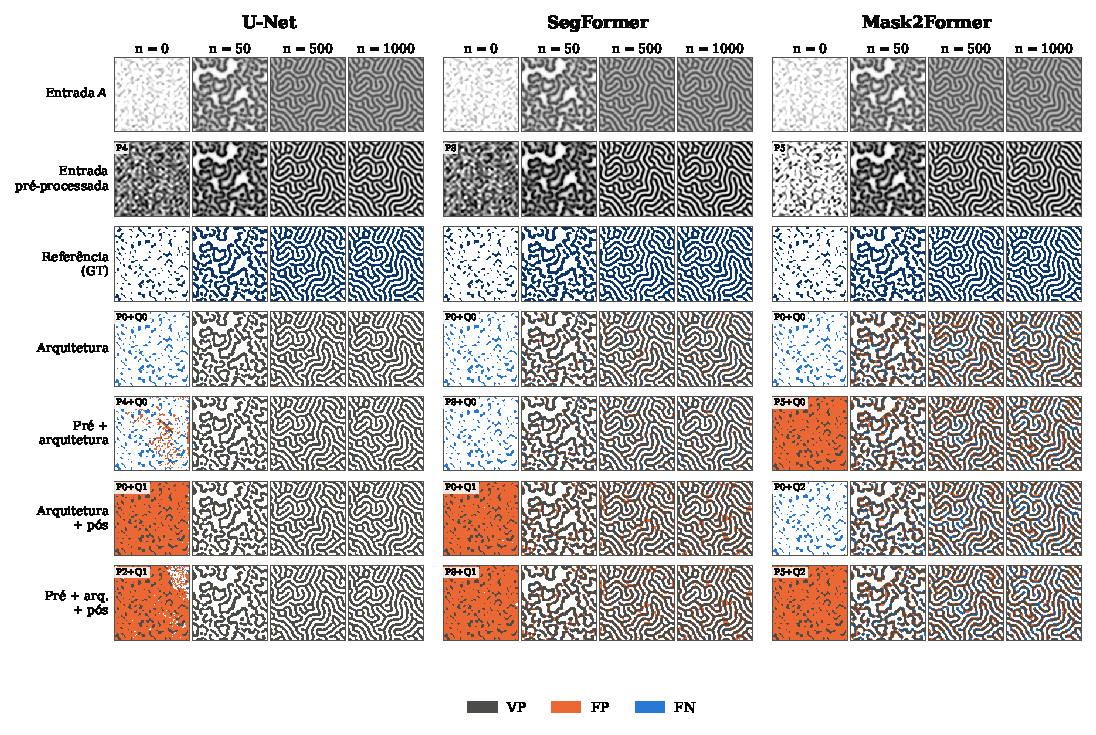
\includegraphics[width=\linewidth]{visual_table_maze}
\caption{Tabela visual do regime \textit{maze}. Mesma organização da Figura~\ref{fig:vt_spirals}.}
\end{figure}

\begin{figure}[htbp]
\centering
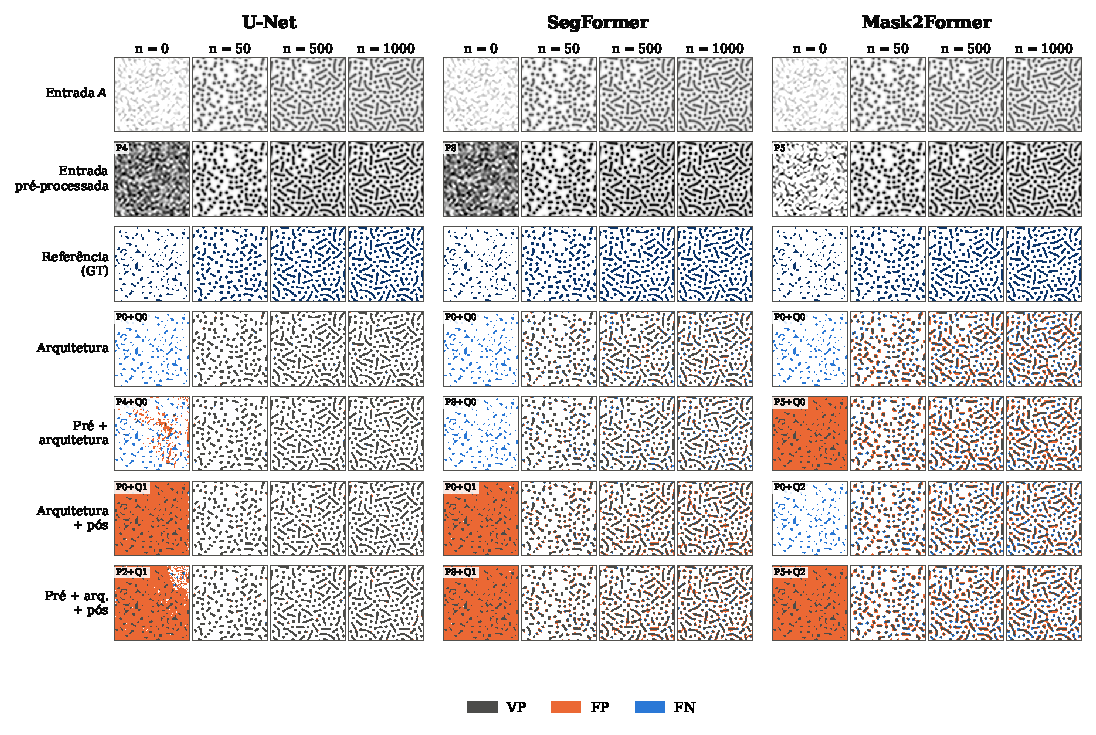
\includegraphics[width=\linewidth]{visual_table_worms}
\caption{Tabela visual do regime \textit{worms}. Mesma organização da Figura~\ref{fig:vt_spirals}.}
\end{figure}

\begin{figure}[htbp]
\centering
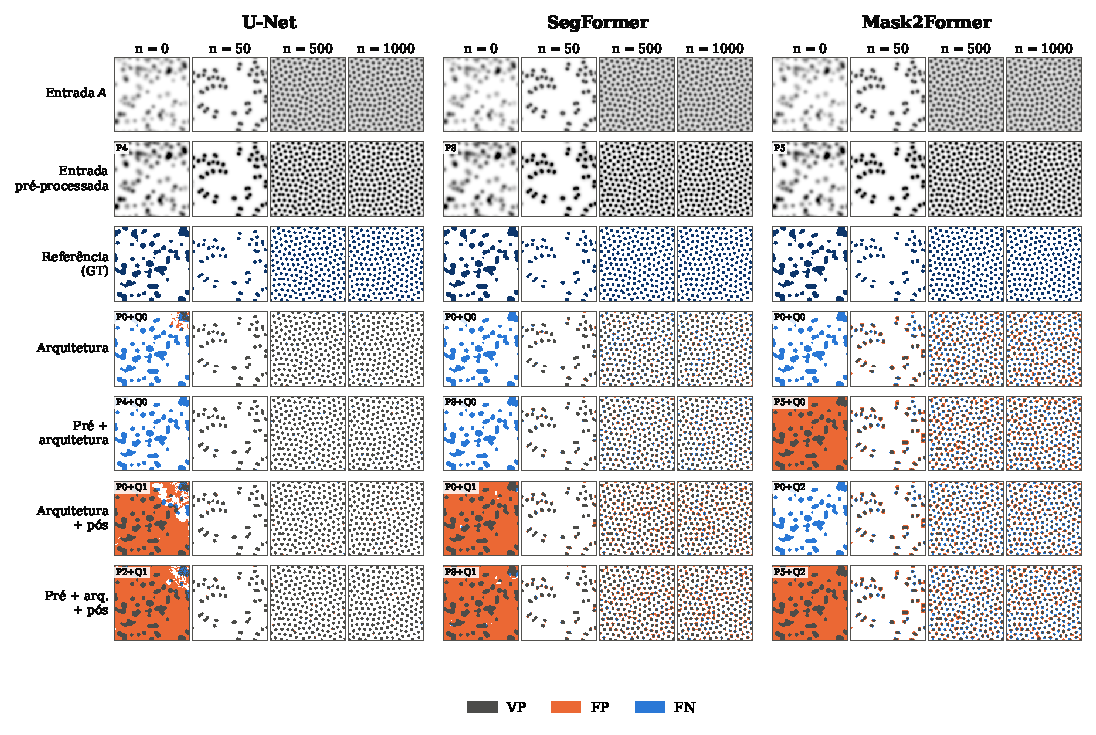
\includegraphics[width=\linewidth]{visual_table_spots}
\caption{Tabela visual do regime \textit{spots}. Mesma organização da Figura~\ref{fig:vt_spirals}.}
\end{figure}

\begin{figure}[htbp]
\centering
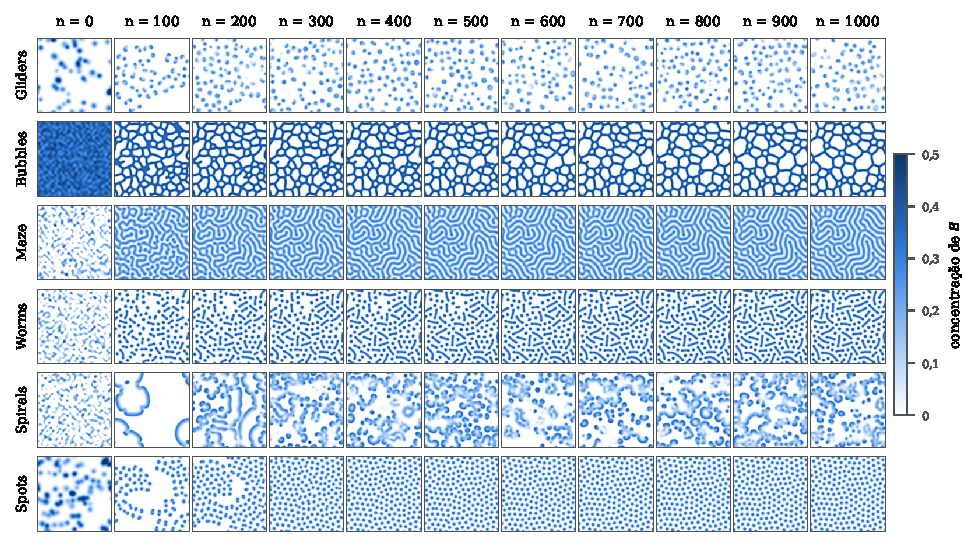
\includegraphics[width=\linewidth]{fluid_by_time}
\caption{Visão geral dos regimes: concentração de $B$ em uma trajetória de teste por regime nos instantes 0 a 1000.}
\label{fig:visao-geral}
\end{figure}

\begin{figure}[htbp]
\centering
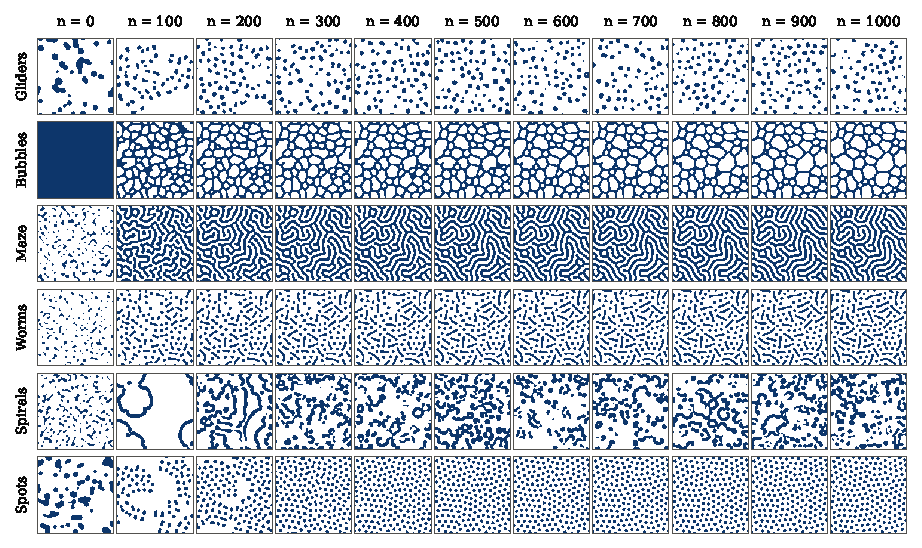
\includegraphics[width=\linewidth]{gt_by_time}
\caption{Referência das mesmas trajetórias, $\ind[B>\tau]$, com o limiar de Otsu do instante 500.}
\end{figure}

\begin{figure}[htbp]
\centering
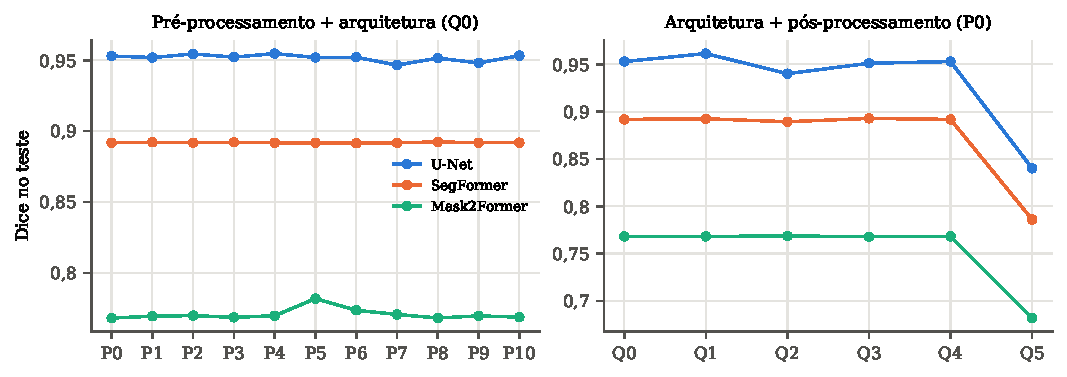
\includegraphics[width=\linewidth]{effects_pre_post}
\caption{Dice no teste por pré-processamento, sem pós-processamento (esquerda), e por pós-processamento, sem pré-processamento (direita).}
\end{figure}

\end{document}
